\documentclass[a4paper,12pt]{article}

% Définition des packages et de leurs paramètres

\usepackage{graphicx}  % Pour insérer des images
\usepackage{textpos}   % Pour positionner précisément les images
\usepackage[french]{babel}  % Utiliser le package babel pour le français
\usepackage{csquotes}         % Ajouter csquotes pour babel
\usepackage[T1]{fontenc}      % Corriger l'encodage pour le français
\usepackage{xcolor}
\usepackage[colorlinks=true, linkcolor=black]{hyperref}  % Liens cliquables en bleu sans les encadrer
\usepackage{amssymb}    % pour les symboles mathématiques
\usepackage{float}      % Pour le placement précis des figures avec [H]
\usepackage{microtype}
\usepackage{caption}
\usepackage{svg}
\svgsetup{inkscape=inkscape}

\usepackage{geometry}  % Pour ajuster les marges
\geometry{top=2cm, bottom=2cm, left=2cm, right=2cm}

% Ajout d'un espace insécable entre les décimales
\usepackage{siunitx}
\sisetup{output-decimal-marker = {,}, group-separator = {\,}, group-minimum-digits = 4}


\usepackage[style=apa, backend=biber]{biblatex}
\addbibresource{references.bib}

\usepackage{tocloft} % Pour modifier l'apparence du sommaire
\setlength{\cftbeforesecskip}{10pt} % Espacement entre les sections
\setlength{\cftbeforesubsecskip}{8pt} % Espacement entre les sous-sections
\renewcommand{\cftsecleader}{\cftdotfill{\cftdotsep}}
\setlength{\cftaftertoctitleskip}{25pt} % Espace sous le titre du sommaire

% Informations du document

\title{Projet Pl@ntNet}
\author{Émilie Aigoin}
\date{January 2025}

\begin{document}

% Logo de l'université en haut à gauche
\begin{textblock*}{3cm}(0.01cm,0.2cm)
    
\includegraphics[width=4cm]{images/Universite.png}
\end{textblock*}

% Logo du master en haut à droite
\begin{textblock*}{3cm}(11cm,1cm)
    
\includegraphics[width=6cm]{images/SSD.png} 
\end{textblock*}

% Titre principal
\vspace{8cm}
\begin{center}
\large{Projet de master présenté dans le contexte de l'UE HAX817X} \\ \vspace{0.4cm}
    {\LARGE \textbf{Prédiction conformelle et base de données \\ \vspace{0.4cm} Pl@ntNet-CrowdSWE}}\\[1cm]
\end{center}

% Logo de l'application centré
\begin{textblock*}{3cm}(5cm,0.5cm)
    
\includegraphics[width=6cm]{images/plantenet.png}
\end{textblock*}

% Informations
\vfill
\begin{center}
Présenté par \\ \vspace{0.2cm}
    {\textbf{AIGOIN Emilie \\ \vspace{0.1cm} CLETZ Laura \\ \vspace{0.1cm} THOMAS Anne-Laure}}\\ \vspace{0.6cm}
    
Sous la direction (ou co-direction) de \\ \vspace{0.2cm}
    {\textbf{BOTELLA Christophe \\ \vspace{0.1cm} SALMON Joseph }}\\ \vspace{1.5cm}
    
    {\large Master Statistique et Science des Données, \\ \vspace{0.1cm} Université de Montpellier}\\ \vspace{0.6cm}
    {\large Année 2024 - 2025}
\end{center}

% Page de garde sans numéro de page
\thispagestyle{empty}

\newpage

% Insertion du sommaire
\tableofcontents 

\newpage

%%%%%%%%%%%%%%%%%%%%%%%%%%%%%%%%%%%%%%%%%%%%%%%%%%%%%%%%%%%%%%%%%%%%%%%%%%%%%%%%
%%%%%%%%%%%%%%%%%%%%%%%%%%%%%%%%%%%%%%%%%%%%%%%%%%%%%%%%%%%%%%%%%%%%%%%%%%%%%%%%

\section{Introduction}

La reconnaissance des plantes est une problématique clé en botanique, avec des applications directes dans la conservation de la biodiversité, la gestion des écosystèmes ou encore la culture personnelle. Parmi les initiatives les plus importantes dans ce domaine, le projet Pl@ntNet joue un rôle central en proposant une application de reconnaissance automatique des plantes basée sur des données collectées par les utilisateurs. Cette approche de science participative permet de constituer une base de données massive et diversifiée de plus de $6$ millions d'observations pour la seule région de l'Europe du Sud-Ouest (SWE), impliquant plus de $\num{800000}$ contributeurs et couvrant plus de $\num{17000}$ espèces végétales. Ce qui est essentiel pour entraîner et affiner les modèles de classification.

\vspace{0.2cm}

Les travaux de recherche sur l'identification automatique des plantes ont considérablement évolué ces dernières années. Initialement, les efforts se sont concentrés sur la comparaison des approches algorithmiques pour maximiser la performance (comme en témoignent les challenges Pl@ntCLEF), puis sur la comparaison avec l'expertise humaine (\cite{Bonnet}). La stratégie dominante consistait alors à accumuler un maximum de données sur un maximum d'espèces pour améliorer l'apprentissage. Cependant, avec l'augmentation constante du nombre d'espèces à identifier et la rareté des données pour la majorité d'entre elles, les performances des systèmes atteignent aujourd'hui certaines limites. Dans ce contexte, quantifier et gérer l'incertitude des prédictions devient un enjeu majeur pour continuer à améliorer les systèmes d'identification automatique des plantes.

\vspace{0.2cm}

Garantir la fiabilité des prédictions et simplifier les sorties utilisateurs reste effectivement un défi majeur. Les données collectées, bien que nombreuses, peuvent être de qualité variable en raison des conditions de prise de vue (lumière, angle, netteté), de la diversité des espèces et de l'expertise variable des contributeurs. Pour améliorer la précision de l'application, il ne suffit pas d’optimiser la classification : nous devons également quantifier l’incertitude des prédictions et adapter dynamiquement la sortie du modèle en fonction du niveau de confiance demandé par l'utilisateur.

\vspace{0.2cm}

Dans ce travail, nous nous sommes intégrées au projet Pl@ntNet avec un objectif précis : améliorer la fiabilité des prédictions en les rendant adaptatives. Plutôt que de fournir une unique réponse avec une probabilité associée ou de fournir un nombre de réponses trop important qui noie l'utilisateur sous trop d'informations, notre objectif était de générer un ensemble de prédictions dont la probabilité de contenir la bonne espèce atteint un niveau de garantie satisfaisant (fixé comme étant $95\%$). Cet ensemble doit être le plus restreint possible pour éviter les suggestions inutiles, tout en s'ajustant automatiquement en fonction de la difficulté de l’identification : être plus précis pour les cas évidents et plus large pour les situations ambiguës.

\vspace{0.2cm}

Pour répondre à cette problématique, nous avons utilisé la prédiction conforme, une approche statistique permettant de transformer les sorties probabilistes d'un modèle de classification en ensembles de prédiction avec des garanties de couverture. Contrairement aux méthodes classiques, la prédiction conforme offre des garanties valides même pour des échantillons de taille finie et sans hypothèses fortes sur la distribution des données (\cite{Angelopoulos}).

\vspace{0.2cm}

Dans la suite de ce rapport, nous détaillerons notre approche en commençant par une présentation approfondie de l'application Pl@ntNet et des données utilisées, suivie d'analyses statistiques descriptives. Nous introduirons ensuite le cadre théorique de la prédiction conforme avant de présenter notre méthodologie, nos résultats principaux et leurs implications pour l'amélioration de l'application.

%%%%%%%%%%%%%%%%%%%%%%%%%%%%%%%%%%%%%%%%%%%%%%%%%%%%%%%%%%%%%%%%%%%%%%%%%%%%%%%%
%%%%%%%%%%%%%%%%%%%%%%%%%%%%%%%%%%%%%%%%%%%%%%%%%%%%%%%%%%%%%%%%%%%%%%%%%%%%%%%%

\section{Jeux de données et outils}

%%%%%%%%%%%%%%%%%%%%%%%%%%%%%%%%%%%%%%%%%%%%%%%%%%%%%%%%%%%%%%%%%%%%%%%%%%%%%%%%

\subsection{Application Pl@ntNet}

Pl@ntNet est un projet de sciences participatives accessible sous forme d’application mobile gratuite, mais également via une \href{https://identify.plantnet.org/fr}{interface en ligne}. Développé conjointement par l'Institut National de Recherche Informatique et Automatique (INRIA), le Centre de coopération International en Recherche Agronomique (CIRAD) et l'Institut de Recherche pour le Développement (IRD), ce projet a été lancé en $2009$ et recense plus de $20$ millions d'utilisateurs dans le monde en $2024$. 

\vspace{0.2cm}

Son objectif principal est d'aider le grand public et les professionnels en botanique à identifier les espèces végétales à partir de photographies. L'application s'appuie sur des algorithmes d'intelligence artificielle qui analysent les caractéristiques visuelles des plantes (écorce, feuilles, fruits, fleurs, etc.) pour proposer des identifications. Au-delà de la reconnaissance des plantes, Pl@ntNet permet également de cartographier la distribution géographique des espèces végétales en fonction de la localisation des photographies partagées par les utilisateurs.

\vspace{0.2cm}

Pl@ntNet est basée sur un principe d’apprentissage coopératif et itératif. Les utilisateurs peuvent partager leurs photographies (que nous appellerons des observations) et celles-ci peuvent être ensuite révisées par la communauté. Cet autre type de contribution est utilisé non seulement pour enrichir la base de données, mais est aussi utilisé par l’IA pour améliorer les performances de son système de reconnaissance. Les utilisateurs peuvent, par exemple, confirmer l'identification d'une espèce, suggérer une identification alternative ou signaler une erreur.

\vspace{0.2cm}

Le processus fonctionne ainsi : lorsqu'un utilisateur soumet une photographie, l'algorithme d'intelligence artificielle analyse l'image et génère une liste d'espèces candidates (appelées étiquettes), chacune associée à une probabilité. L'espèce affichée en première position est celle que l'intelligence artificielle estime la plus probable, suivie des autres classées par ordre décroissant de probabilité. Pour garantir la pertinence des suggestions et ne pas surcharger l'utilisateur d'informations avec des espèces peu probables, l'affichage est limité aux espèces dont la probabilité dépasse le seuil minimal, fixé à $0,001$ (soit $0,1\%$).

\vspace{0.2cm}

Notre travail est basé sur une démarche d'optimisation de ce système, avec pour objectif de rendre le nombre d'étiquettes présentées adaptatif à la difficulté du problème d'identification : plus l'identification est facile, moins le système proposera d'options à l'utilisateur, et inversement pour les cas ambigus ou difficiles.

\vspace{0.2cm}

Toutes les interactions entre les utilisateurs et le système (incluant les images soumises, les prédictions de l'intelligence artificielle et les validations humaines) sont stockées dans une base de données qui a constitué notre jeu de données tout au long de ce projet.

%%%%%%%%%%%%%%%%%%%%%%%%%%%%%%%%%%%%%%%%%%%%%%%%%%%%%%%%%%%%%%%%%%%%%%%%%%%%%%%%

\subsection{Présentation du jeu de données}

Notre étude s'est appuyée sur plusieurs jeux de données extraits de Pl@ntNet. Ces extractions de la base, normalement non-accessible au public et organisée de manière relativement complexe, ont été rendues accessibles principalement à des fins de recherche et présentent, plus clairement et intuitivement, chacune des caractéristiques spécifiques en termes de taille, de structure et de variables, qui comprennent en sus les annotations des utilisateurs.

\vspace{0.2cm}

Dans un premier temps, nous nous sommes familiarisées avec le jeu de données principal Pl@ntNet-CrowdSWE (pour South-West Europe), comprenant $\num{6 699 593}$ observations d'espèces végétales situées en Europe du Sud-Ouest. Ces observations ont été réalisées par $\num{823 251}$ utilisateurs de l'application Pl@ntNet, parmi lesquels nous distinguons deux catégories : 
\begin{itemize}
    \item \textbf{Les experts :} au nombre de $98$, ce sont des botanistes professionnels ou des amateurs très expérimentés dont nous admettons la véracité des identifications.
    \item \textbf{Les non-experts :} constituent la majorité des contributeurs et comprennent tous les utilisateurs novices en botanique.
\end{itemize}

\vspace{0.2cm}

Cette distinction est très importante pour notre approche, car les identifications fournies par les experts servent de vérité terrain pour évaluer la qualité des prédictions automatiques et pour calibrer notre modèle de prédiction conforme.

\vspace{0.2cm}

Les données contiennent les variables suivantes :
\begin{itemize}
    \item Les identifiants uniques pour chaque utilisateur (avec leur expertise précisée).
    \item Les identifiants uniques pour chaque observation.
    \item Les identifiants pour chaque espèce (un identifiant spécifique pour ceux dans la base de données mondiale et un identifiant spécifique pour ceux dans la base de données SWE).
    \item Les noms scientifiques complets des espèces.
    \item Les prédictions générées par l'algorithme d'intelligence artificielle pour chaque observation avec leurs probabilités associées.
    \item Les métadonnées sur les images (date, localisation, type d'organe photographié).
    \item Les votes des utilisateurs sur les identifications et leurs propositions sur les observations.
\end{itemize}

\vspace{0.2cm}

Le tableau ci-dessous résume les principales caractéristiques de ce jeu de données :

\vspace{0.2cm}

\begin{table}[H]
\centering
\begin{tabular}{|l|r|}
    \hline
    \textbf{Caractéristique} & \textbf{Valeur} \\
    \hline
    Zone géographique  & Europe du Sud-Ouest  \\
    Nombre d'observations & $\num{6 699 593}$  \\
    Nombre d'observations expertes & $\num{26 501}$ \\
    Nombre d'utilisateurs  & $\num{823 251}$  \\
    Nombre d'utilisateurs experts  & $98$  \\
    Nombre d'espèces observées  & $\num{17 247}$  \\
    Période couverte  & $2015-2023$  \\
    \hline
    \end{tabular}
\caption{Caractéristiques principales du jeu de données Pl@ntNet-CrowdSWE}
\label{tab:recap des caractéristiques}
\end{table}
    
\vspace{0.2cm}

Ces données sont réparties dans $7$ fichiers au format JSON (JavaScript Object Notation) et $2$ fichiers textes disponibles sur la \href{https://zenodo.org/records/10782465}{plateforme Zenodo}, un centre de données du CERN ouvert à tous.

\vspace{0.2cm}

Dans un deuxième temps, nous avons travaillé avec un échantillon plus restreint de $\num{67 466}$ observations afin de faciliter le développement et les tests de nos algorithmes, permettant une exécution plus rapide qu'avec l'ensemble complet des $7$ millions de données. Cette approche nous a permis d'itérer efficacement sur nos modèles avant de les généraliser, dans un dernier temps, sur l'intégralité du jeu de données.

\vspace{0.2cm}

À partir de ces données, notre première tâche a consisté à croiser les différents tableaux pour créer un jeu de données unifié contenant toutes les informations nécessaires pour chaque observation. Pour cette fusion, nous avons privilégié le croisement basé sur les identifiants numériques des espèces plutôt que par le nom scientifique dans un but de gain de temps de traitement. Nous avons réalisé ces croisements à l'aide de plusieurs outils.

%%%%%%%%%%%%%%%%%%%%%%%%%%%%%%%%%%%%%%%%%%%%%%%%%%%%%%%%%%%%%%%%%%%%%%%%%%%%%%%%

\subsection{Outils}

Pour mener à bien nos analyses, nous avons développé une chaîne de traitements combinant plusieurs langages et outils de programmation. Tous nos codes sont disponibles en libre accès sur notre \href{https://github.com/lcletz/PLANTNET_M1_SSD}{Github} ainsi que les données partagées entre nous au fur et à mesure de l'étude sur la plateforme Zenodo : l'ensemble des \href{https://zenodo.org/records/15355864}{données post-traitement}, les \href{https://zenodo.org/records/15353081}{scores} calculées sur les données traitées qui ont en suite été divisées en \href{https://zenodo.org/records/15358242}{non-experts} et \href{https://zenodo.org/records/15441471}{experts}.

\subsubsection{Environnement de développement}

Nous avons principalement utilisé les langages de programmation R via RStudio (\cite{RStudio}) ainsi que Python (\cite{Python}) pour le traitement des données et les analyses statistiques. Le fait d'avoir utilisé plusieurs langages nous a permis de tirer parti de leurs forces : R pour ses capacités graphiques et statistiques avancées et Python pour sa flexibilité dans la manipulation de grands volumes de données (possibilités de travailler avec des fichiers zippés).

\subsubsection{Bibliothèques R}

Pour nos analyses sous R, nous avons mobilisé les packages suivants :
\begin{itemize}
    \item \textbf{Manipulation des données :} \texttt{jsonlite} pour la lecture et l'écriture de fichiers JSON, \texttt{tibble} et \texttt{data.table} pour optimiser le traitement de grands tableaux de données, \texttt{dplyr} et \texttt{tidyr} pour les opérations de filtrage et de croisements de données.
    \item \textbf{Visualisation :} \texttt{ggplot2} pour la création de graphiques, \texttt{gridExtra} pour la composition de plusieurs graphiques, \texttt{htmlwidget} et \texttt{plotly} pour générer des visualisations interactives exportables.
    \item \textbf{Traitement fonctionnel :} \texttt{purrr} pour appliquer des fonctions prenant en entrée des vecteurs dans les listes larges, \texttt{stringr} pour manipuler des chaînes de caractères.
    \item \textbf{Repérage temporel :} \texttt{progress} pour chronométrer et estimer la durée des algorithmes.
\end{itemize}

\subsubsection{Bibliothèques Python}

Pour nos analyses sous Python, les bibliothèques dont nous avons fait usage sont :
\begin{itemize}
    \item \textbf{Gestion de fichiers :} \texttt{requests}, \texttt{io}  et \texttt{zipfile} pour la récupération et extraction de fichiers compressés, \texttt{json} et \texttt{tarfile} pour la manipulation de fichiers JSON et TAR (archives compressées), \texttt{os} et \texttt{glob} pour la navigation et la recherche dans l'arborescence des fichiers.
    \item \textbf{Analyse de données :} \texttt{pandas} pour la manipulation tabulaire des données et les opérations de fusion, \texttt{numpy} pour les calculs numériques vectorisés.
    \item \textbf{Visualisation :} \texttt{matplotlib pyplot}, \texttt{seaborn} pour la création de graphiques et \texttt{plotly express(px)} pour créer des graphiques interactifs.
    \item \textbf{Optimisation :} \texttt{tqdm} pour suivre visuellement la progression des traitements, \texttt{math} pour utiliser des fonctions mathématiques avancées.
    \item \textbf{Aléatoire :} \texttt{random} pour mélanger et diviser les données de manière aléatoire mais reproductible.
    \item \textbf{Exportation de graphique :} \texttt{kaleido} qui est une bibliothèque pour exporter des graphiques issus de \texttt{plotly} en images statiques.
\end{itemize}

\vspace{0.2cm}

Cette complémentarité des outils nous a permis d'aborder efficacement les différentes phases du projet : de l'exploration initiale des données à l'implémentation des algorithmes de prédiction conformes, en passant par la visualisation des résultats.

%%%%%%%%%%%%%%%%%%%%%%%%%%%%%%%%%%%%%%%%%%%%%%%%%%%%%%%%%%%%%%%%%%%%%%%%%%%%%%%%

\subsection{Pré-traitement des données}

Dans le contexte de notre projet sur Pl@ntNet, nous avons dû adapter la méthode standard pour tenir compte de plusieurs spécificités. 

\vspace{0.2cm}

Une étape importante consistait à établir une vérité terrain fiable pour chaque observation, c'est-à-dire à déterminer quel label était le vrai pour chaque observation. Pour les observations avec le vote d'un utilisateur expert, nous avons directement utilisé leur identification comme référence absolue. Pour les observations sans validation experte, nous avons appliqué une méthode de vote majoritaire parmi les identifications fournies par les utilisateurs. C'est-à-dire que nous avons compté le nombre de réponses par label donné, en donnant un poids plus important à l'utilisateur ayant pris la photo (poids égal à $3$), car c'est le seul à avoir réellement vu la plante, et avons posé que c'était l'espèce avec le plus de votes qui était le label correct. En cas d'égalité entre deux espèces candidates, nous avons sélectionné aléatoirement l'une d'entre elles.

\vspace{0.2cm}

Ces données séparées, nous avons pu lancer le premier algorithme de pré-traitement de celles-ci dont le but est de chercher dans chaque liste d'espèces, pour chaque observation, le label considéré comme la vérité terrain.

\vspace{0.2cm}

Comme les listes que nous avons récupérées étaient tronquées, ne conservant que les espèces dont la probabilité prédite est supérieure à un certain seuil ($1/1000$), nous avons décidé de considérer que les classes non présentes dans la liste avaient une probabilité de $1/1000$, ce qui nous a permis d'appliquer les formules de scores décrites dans la prochaine section sans souci.

\vspace{0.2cm}

Ces adaptations nous ont permis d'appliquer avec succès le cadre de prédiction conforme à notre problématique d'identification des plantes, pour pouvoir par la suite déterminer nos ensembles de prédiction.

%%%%%%%%%%%%%%%%%%%%%%%%%%%%%%%%%%%%%%%%%%%%%%%%%%%%%%%%%%%%%%%%%%%%%%%%%%%%%%%%

\section{Analyses}

%%%%%%%%%%%%%%%%%%%%%%%%%%%%%%%%%%%%%%%%%%%%%%%%%%%%%%%%%%%%%%%%%%%%%%%%%%%%%%%%

\subsection{Statistiques descriptives}

Bien avant de nous atteler aux analyses plus poussées comme les algorithmes de prédiction conforme ou les calculs des scores, nous avons réalisé une série de statistiques descriptives sur les premiers jeux de données. Ces analyses préliminaires nous ont permis de mieux comprendre la nature des données et d'identifier certains phénomènes intéressants.

\subsubsection{Distribution des espèces observées}

Nous avons tout d'abord examiné la répartition des espèces "Top 1" en Europe du Sud-Ouest. Ce que nous appelons le "Top 1" est l'espèce qui apparait en tête des probabilités prédites par l'algorithme de l'application après que la photographie a été prise. Cette position traduit la certitude de l'IA en la reconnaissance de l'espèce et, s'il s'avère que c'est la bonne prédiction, alors cela reflète également la qualité des prédictions pour cette espèce. Nous allons considérer dans un premier temps qu'il s'agit là de la vérité observée, donc la bonne espèce photographiée, et étudions sa répartition :

\begin{figure}[H]
    \centering
    \includesvg[height=10cm]{images/figure1.svg}
    \caption{Histogramme du nombre d'observations par espèce avec les 10 espèces les plus observées et 5 des moins observées}
    \label{fig1}
\end{figure}

Comme le montre la \hyperref[fig1]{\textcolor{purple}{figure 1}}, les espèces "Top 1" les plus fréquentes, dont nous allons dire qu'elles sont les plus fréquemment photographiées par les utilisaeur de Pl@ntNet, sont essentiellement des arbres vivaces, certains fruitiers, ou des fleurs comestibles, aux propriétés curatives et qui peuvent être aperçues dans toute la zone géographique étudiée. Le \textit{Prunus Spinosa L.} (\hyperref[fig:prunus]{\textcolor{purple}{figure 3}}) ou, plus communément, prunellier, arrive en tête des observations, suivi par d'autres espèces communes comme le \textit{Fagus Sylvatica L.} (hêtre commun) ou encore le \textit{Corylus avellana L.} (noisetier commun). Cette distribution n'est pas surprenante puisqu'elle reflète à la fois l'abondance de ces espèces et l'intérêt qu'elle suscite auprès du grand public, soit pour leur valeur décorative, soit pour leurs usages alimentaires ou médicinaux.

\vspace{0.2cm}

À l'autre extrémité, les espèces les moins observées (avec une seule occurrence dans la base) correspondent généralement à des plantes rares, présentes dans des zones très restreintes ou éloignées de l'Europe du Sud-Ouest, ou simplement moins reconnaissables et moins intéressantes aux yeux du public. Nous comptons par exemple le \textit{Pavonia Spinifex (L.) Cav.} (\hyperref[fig:prunus]{\textcolor{purple}{figure 3}}), un arbuste à fleurs jaunes originaire des Caraïbes, le \textit{Citrus paradisi Macfad.}, un agrume hybride communément appelé "pomélo" ou le \textit{Teucrium murcicum Sennen}, une toute petite herbe méditerranéenne.

\subsubsection{Relation entre fréquence d'observation et probabilités}

Au-delà de la simple fréquence d'apparition de ces espèces, qui semble seulement impliquer un intérêt de l'observateur, nous nous sommes intéressées à la relation entre cette fréquence et la qualité des prédictions de l'algorithme d'intelligence artificielle, et donc ces fameuses probabilités associées à l'espèce "Top 1".  Nous avons obtenu les graphiques suivants :

\begin{figure}[H]
\centering
\begin{minipage}{0.5\textwidth}
  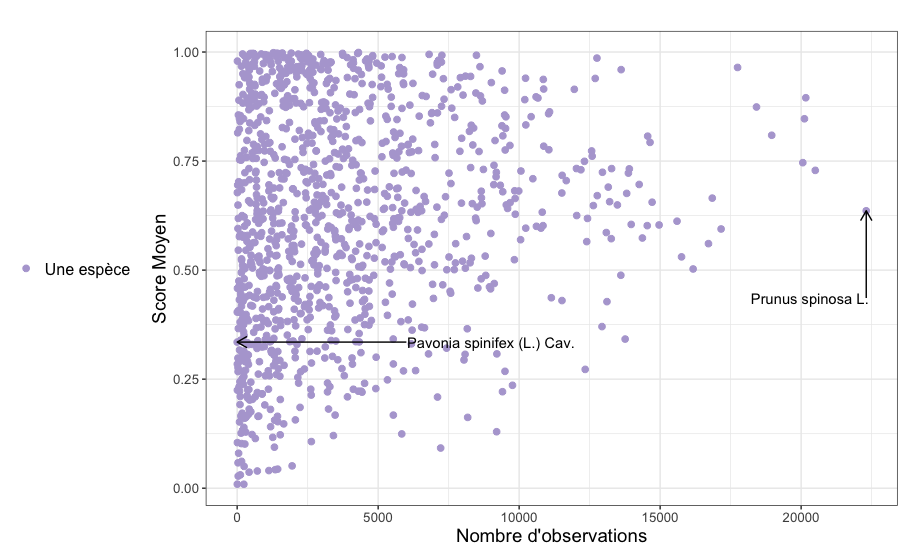
\includegraphics[width=0.9\linewidth]{images/mean_rd.png}
\end{minipage}%
\begin{minipage}{0.5\textwidth}
  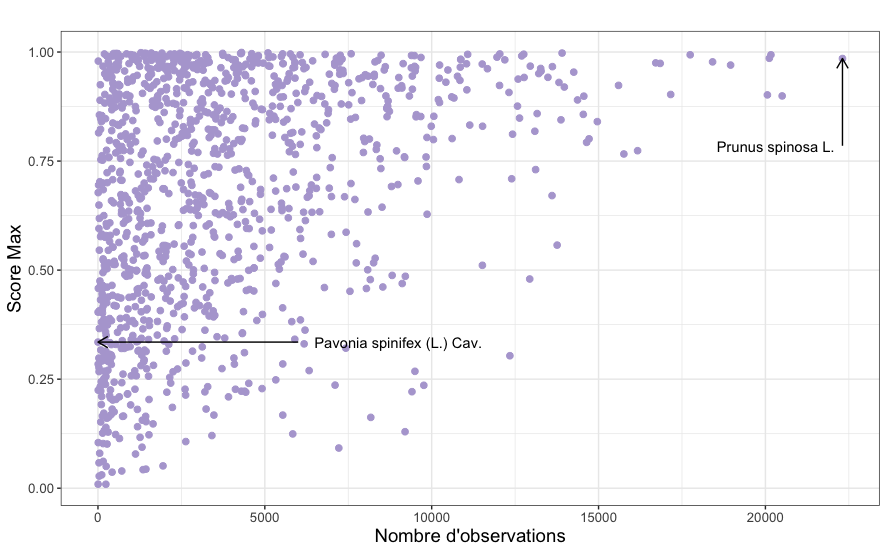
\includegraphics[width=0.9\linewidth]{images/max_rd.png}
\end{minipage}
\caption{Nuages de points de la moyenne des scores ou des scores max en fonction du nombre d'observations}
\end{figure}

Ces deux graphes, comptant environ $\num{1100}$ espèces distinctes désignées aléatoirement, révèlent plusieurs phénomènes intéressants. Nous les constaterons grâce à cette répartition des scores en fonction du nombre d'observations par espèces.

\vspace{0.2cm}

Contrairement à ce que nous pourrions intuitivement penser, il n'existe pas de relation linéaire évidente entre la fréquence d'observation d'une espèce et la confiance moyenne du système dans ses prédictions. Des espèces très fréquentes peuvent recevoir des scores moyens relativement bas, tandis que certaines espèces rares obtiennent des scores élevés. Les probabilités sont éparses, l'algorithme n'est pas systématiquement confiant : il renvoit sûrement plusieurs espèces ayant des scores voisins en "Top 2", "Top 3", etc. sur lesquels nous devrons nous pencher.

\vspace{0.2cm}

Le \textit{Prunus Spinosa L.}, l'espèce la plus observée, présente un score moyen relativement élevé (proche de $0,6$), ce qui suggère que le système est généralement confiant dans son identification. Cela peut s'expliquer par ses caractéristiques morphologiques distinctives et possiblement par la qualité généralement bonne des photos de cette espèce commune.

\vspace{0.2cm}

Certaines espèces n'ayant qu'une seule observation présentent des scores très élevés, proches de $1$. Ce phénomène pourrait s'expliquer par le processus d'apprentissage du modèle : si l'intelligence artificielle a été entraînée sur des images similaires à cette unique observation dans notre jeu de données, elle peut la reconnaître avec une grande confiance. Nous pouvons tout à fait le discerner sur les précédents graphes puisque le \textit{Pavonia Spinifex (L.) Cav.} a vu s'être attribué une probabilité autour de $0,35$, ce qui est plutôt correct pour une espèce n'appartenant normalement pas à la flore d'Europe du Sud-Ouest.

%%%%%% PAVONIA SPINIFEX : https://identify.plantnet.org/fr/k-world-flora/species/Pavonia%20spinifex%20%28L.%29%20Cav./data %%%%%%
%%%%%% PRUNUS SPINOSA : https://identify.plantnet.org/fr/k-world-flora/species/Prunus%20spinosa%20L./data %%%%%%

\begin{figure}[H]
\centering
\begin{minipage}{0.5\textwidth}
  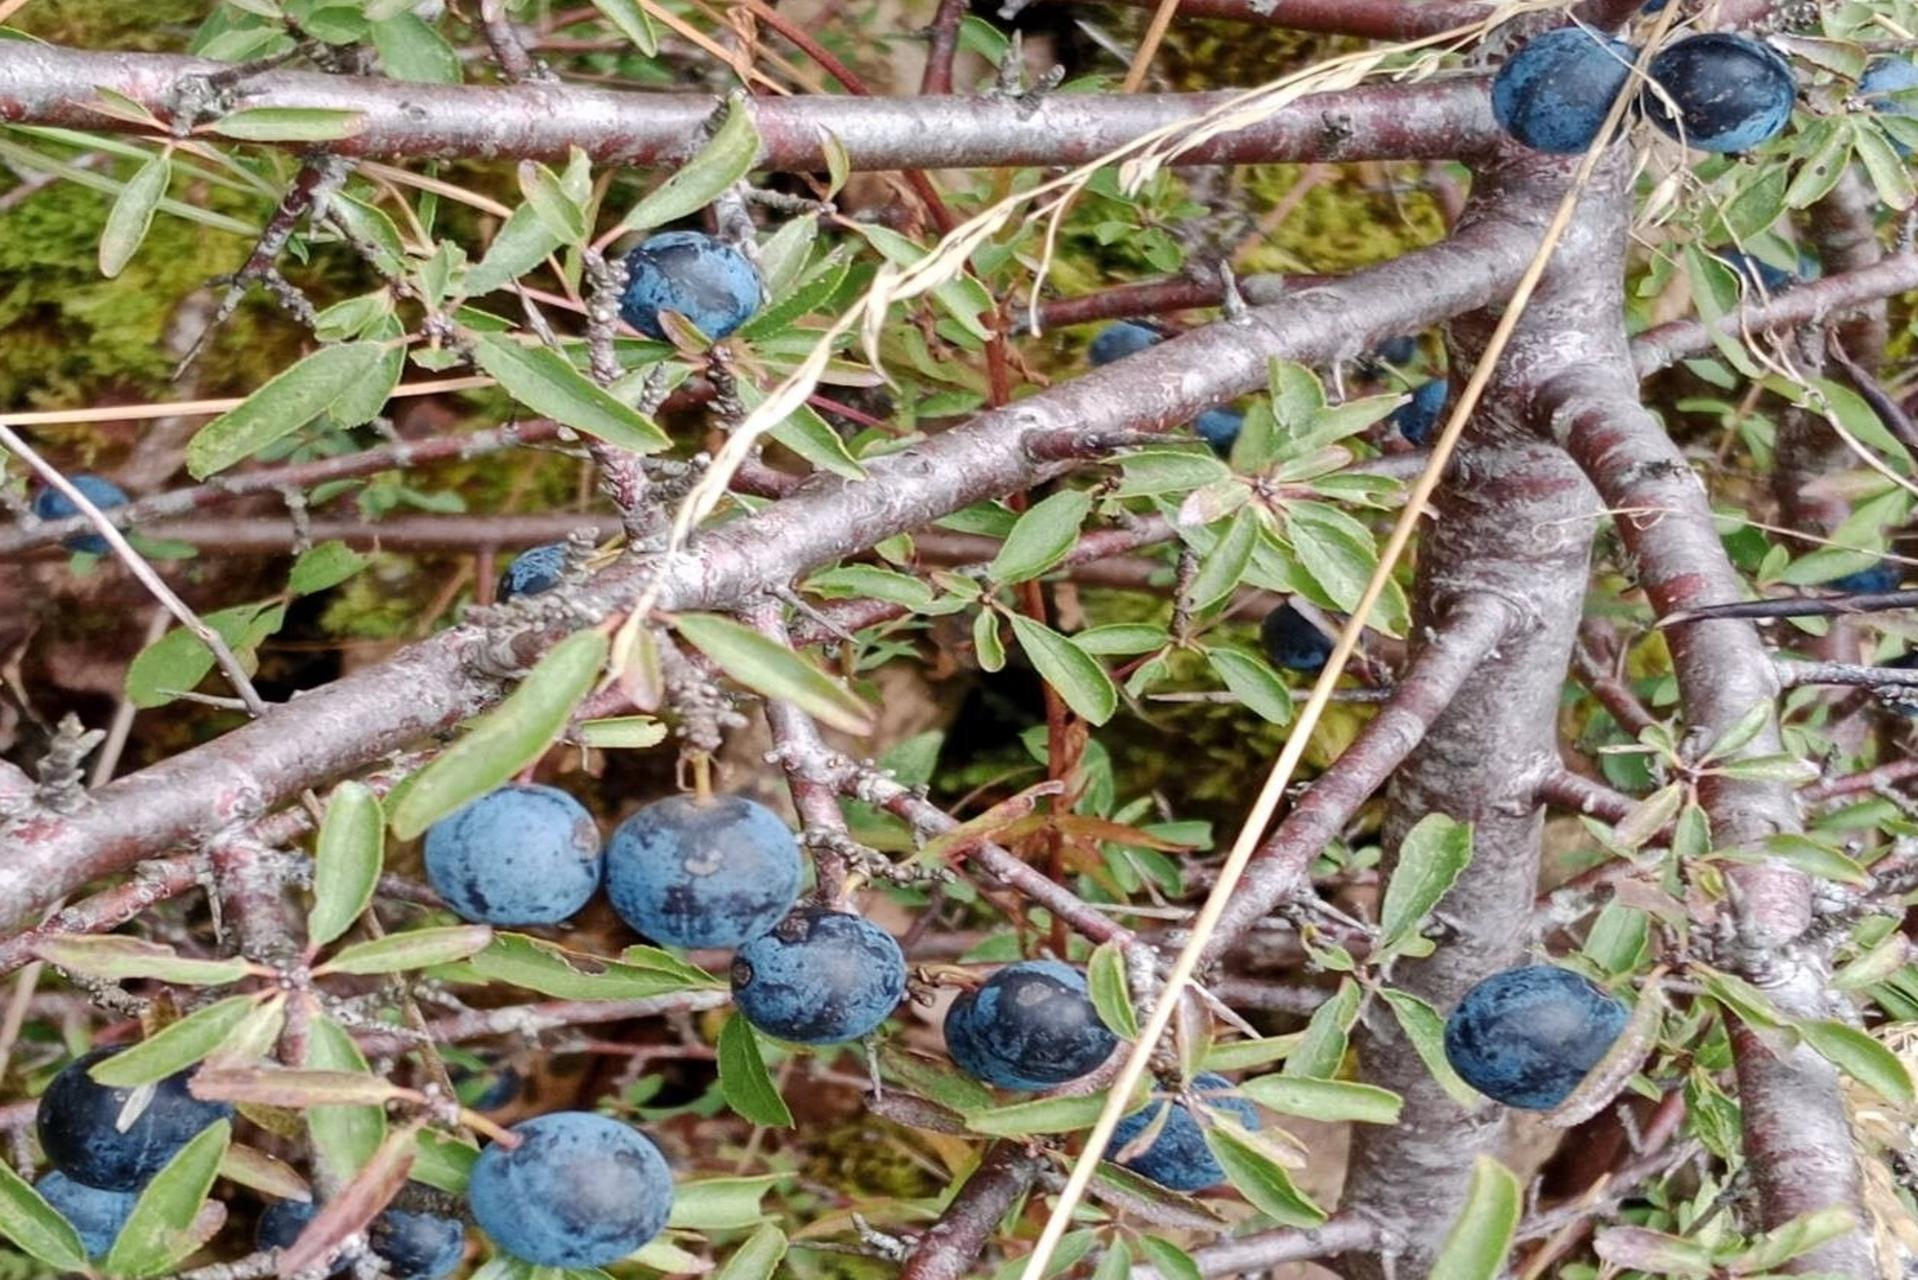
\includegraphics[width=0.9\linewidth]{images/prunus_spinosa.jpeg}
\end{minipage}%
\begin{minipage}{0.5\textwidth}
  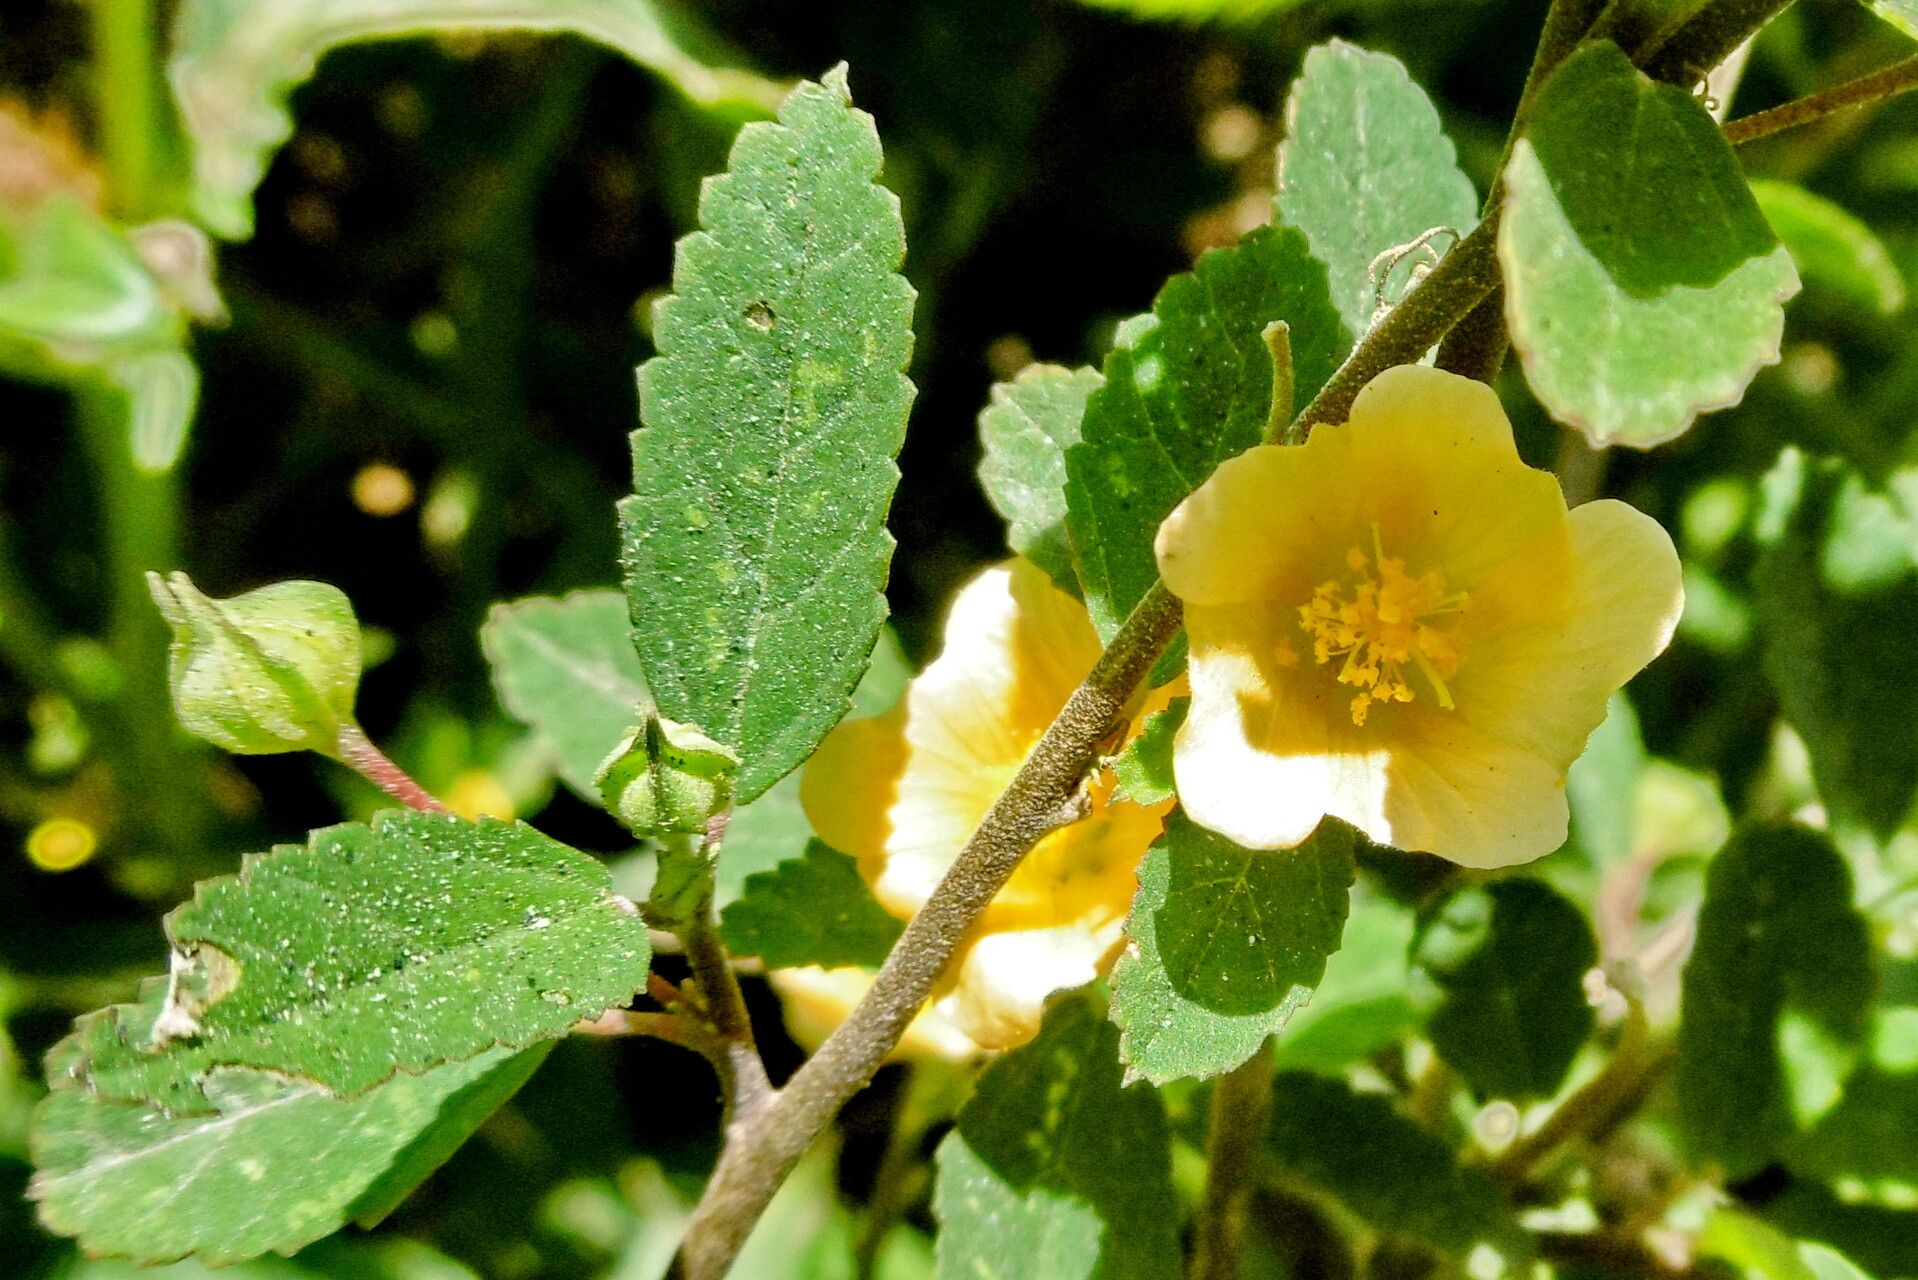
\includegraphics[width=0.9\linewidth]{images/pavonia_spinifex.jpeg}
\end{minipage}
\caption{Prunus Spinosa L. et Pavonia Spinifex (L.) Cav.}
\label{fig:prunus}
\end{figure}

\subsubsection{Facteurs influençant la qualité des prédictions}

Plusieurs facteurs peuvent expliquer la variabilité observée dans les scores de prédiction : 
\begin{itemize}
    \item \textbf{Qualité des images :} les photos floues, mal cadrées, prises de trop loin ou dans des conditions d'éclairage défavorables réduisent considérablement la performance de l'algorithme.
    \item \textbf{Confusion entre espèces similaires :} certaines espèces appartenant au même genre partagent des caractéristiques morphologiques très proches, ce qui peut induire l'algorithme en erreur. Par exemple, différentes espèces de chênes ou de roses peuvent être difficiles à distinguer même pour des botanistes expérimentés.
    \item \textbf{Stade de développement de la plante :} une même espèce peut présenter des aspects très différents selon la saison (avec ou sans feuilles, en fleur ou non, avec ou sans fruit, etc.), ce qui peut affecter la confiance du système dans ses prédictions.
    \item \textbf{Organe photographié :} les fleurs sont généralement plus distinctives et permettent une identification plus fiable que les feuilles ou les tiges, qui peuvent présenter plus de similarités entre espèces.
    \item \textbf{Effet d'apprentissage sur des images spécifiques :} comme mentionné précédemment, certaines espèces rares peuvent obtenir des scores très élevés si l'image soumise est similaire à celle utilisée pour l'entraînement du modèle.
\end{itemize}

\subsubsection{Impact du choix de l'utilisateur}

Les espèces associées aux probabilités "Top 1" ne sont pas systématiquement celles choisies par l'observateur, qui peut décider de désigner une espèce de probabilité plus faible également proposée par l'IA ou opter pour une tout autre espèce. Des utilisateurs n'ayant pas observé eux-mêmes, sur place, peuvent également choisir une espèce à l'instar de l'observateur. Nous avons admis l'espèce correcte par vote majoritaire où l'observateur a plus de poids que les autres votants. Nous allons étudier un échantillon de $\num{67 461}$ observations (environ un centième des données totales). Observons sur cet échantillon les différences entre le "Top 1" (\hyperref[fig1]{\textcolor{purple}{figure 1}}) et le vote majoritaire (\hyperref[fig4]{\textcolor{purple}{figure 4}}).

\vspace{-0.4cm}

\begin{figure}[H]
    \centering
    \includesvg[height=10cm]{images/figure3.svg}
    \caption{Histogramme du nombre d'observations par espèce avec les 6 espèces les plus choisies et 4 des moins choisies}
    \label{fig4}
\end{figure}

\vspace{0.2cm}

Si \textit{Prunus Spinosa L.} est toujours présente dans ce graphique, c'est l'espèce \textit{Malva sylvestris L.} (\hyperref[fig:malva]{\textcolor{purple}{figure 6}}), une fleur au mauve intense, qui est en tête. Elle est donc la plus souvent choisie par les utilisateurs pour cet échantillon. Ce graphique seul indique que l'espèce prédite en première par l'intelligence artificielle, celle en qui l'algorithme est le plus confiant, n'est pas toujours ce que l'utilisateur compte choisir. Il est envisageable que les espèces proposées par l'inteligence artificielle dans son "Top K" se ressemblent : il existe par exemple plusieurs espèces d'iris ou de lotus partageant donc des caractéristiques communes, on parle de "familles".

\vspace{0.2cm}

Parmi les espèces les moins choisies par les utilisateurs dans cet échantillon, nous notons la \textit{Daphne striata Tratt.} (\hyperref[fig:malva]{\textcolor{purple}{figure 6}}), un arbrisseau à fines fleurs roses produisant des baies qui ressemblent à des œufs, le \textit{Crepis bursifolia L.}, une fleur jaune courante dans l'Hérault et le Var mais qui ne s'observe que vers Mai-Juin, ou le \textit{Cencrhus setaceus (Forssk.) Morrone}, une herbe envahissante dans toute l'Afrique. Ce sont des espèces faciles à reconnaître mais peu courantes.

\begin{figure}[H]
    \centering
    \begin{minipage}{0.5\textwidth}
      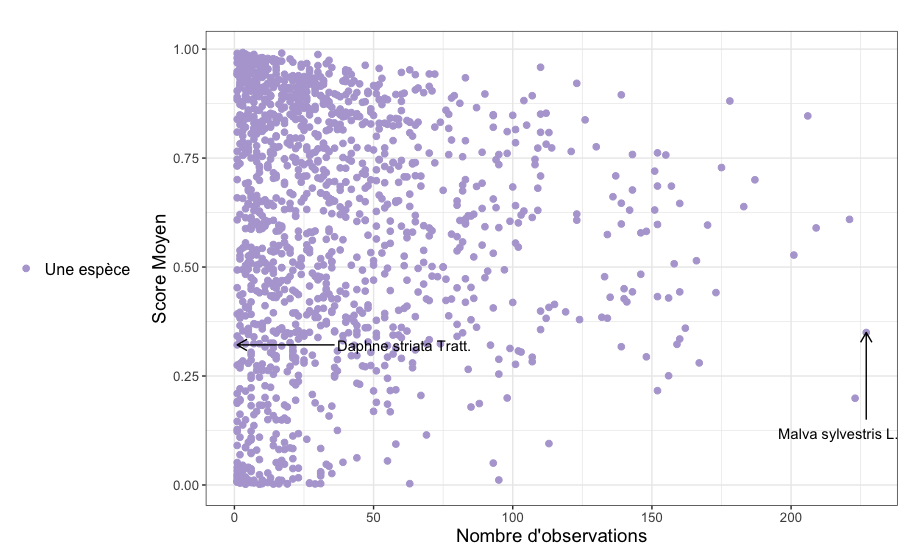
\includegraphics[width=0.9\linewidth]{images/mean_rd_users.png}
    \end{minipage}%
    \begin{minipage}{0.5\textwidth}
      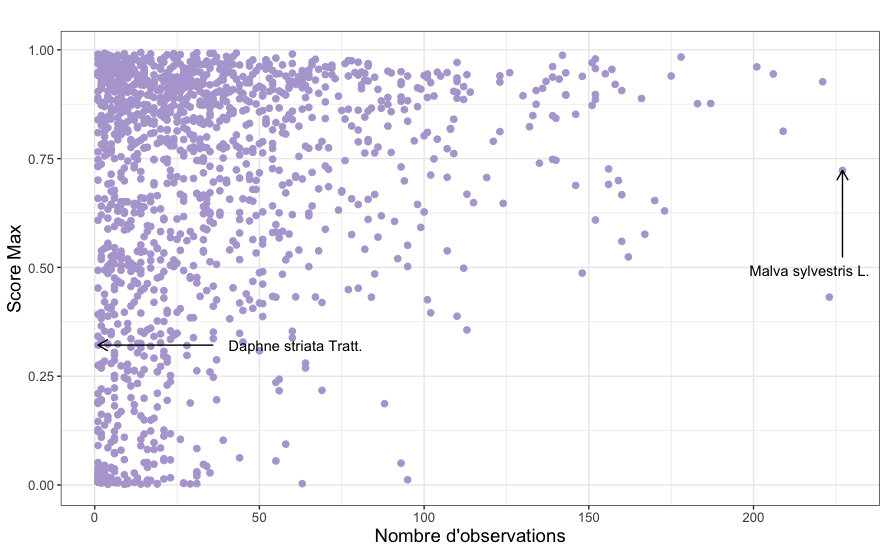
\includegraphics[width=0.9\linewidth]{images/max_rd_users.png}
    \end{minipage}
    \caption{Nuages de points de la moyenne des scores ou des scores max en fonction du nombre d'observations}
\end{figure}


Puisque l'échantillon étudié est moins conséquent que celui de la première étude, environ 1400 espèces ont été piochées aléatoirement, soit trois centaines supplémentaires, pour une meilleure intuition. 
\vspace{0.2cm}

La Mauve, choisie plus de $200$ fois dans cet échantillon, possède en moyenne une probabilité assez basse. Cela suggère qu'elle n'a pas toujours été l'espèce Top $1$ mais qu'elle a tout de même été validée par l'observateur ou par les votants à la majorité. Lorsqu'elle a été proposée par l'algorithme, même si elle n'était pas en première position ni avec une probabilité élevée, l'observateur a toutefois opté pour cette espèce. Cela pourrait s'expliquer par le fait que cette plante est d'une couleur intense et d'une forme assez particulière que l'observateur a pu remarquer et facilement reconnaître.

\vspace{0.2cm}

Une des plantes n'ayant été choisie qu'une seule fois dans cet échantillon est la \textit{Daphne striata Tratt.}. Son score est pourtant assez bas, nous pouvons imaginer qu'elle n'était proposée par l'application qu'en deuxième ou troisième position. Comme cité plus tôt, c'est un curieux arbrisseau qui est facile à identifier par l'observateur donc ce dernier a pu la choisir sans trop d'hésitation malgré le manque de confiance de l'IA.

\vspace{0.2cm}

Outre ces deux espèces, nous remarquons qu'il y a plusieurs espèces aux scores très proches de $0$ qui ont été choisies, soit parce que l'intelligence artificielle n'était pas confiante et a proposée de nombreuses options ayant des probabilités minimes, soit parce que les votants ont choisi une espèce en particulier parmi les espèces les moins évidentes selon l'IA.

%%%%% MALVA SYLVESTRIS : https://identify.plantnet.org/k-world-flora/species/Malva%20sylvestris%20L./data#galleries %%%%%
%%%%% DAPHNE STRIATA : https://identify.plantnet.org/fr/k-world-flora/species/Daphne%20striata%20Tratt./data#galleries %%%%%

\begin{figure}[H]
    \centering
    \begin{minipage}{0.5\textwidth}
      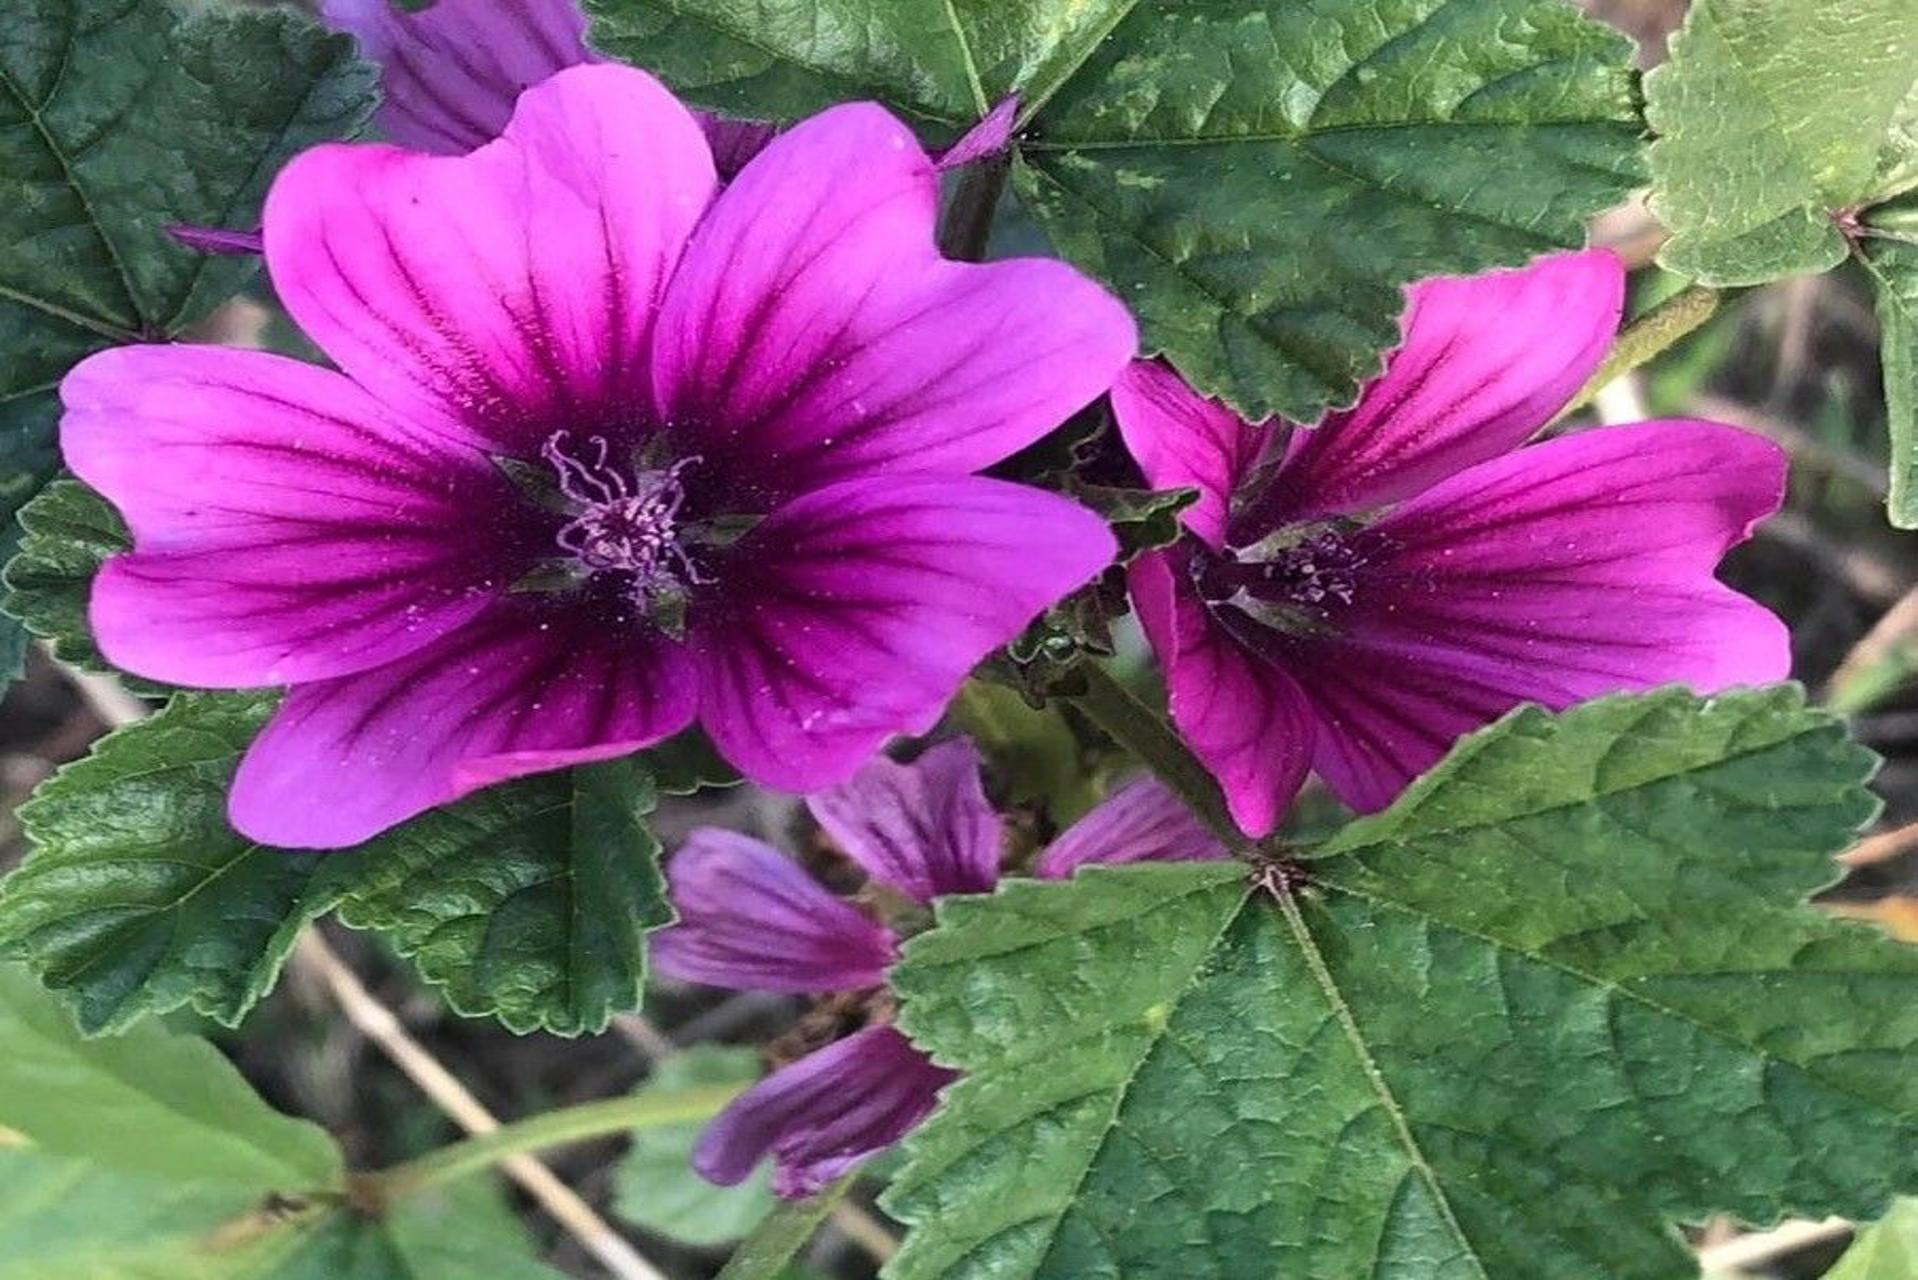
\includegraphics[width=0.9\linewidth]{images/malva_sylvestris.jpeg}
    \end{minipage}%
    \begin{minipage}{0.5\textwidth}
      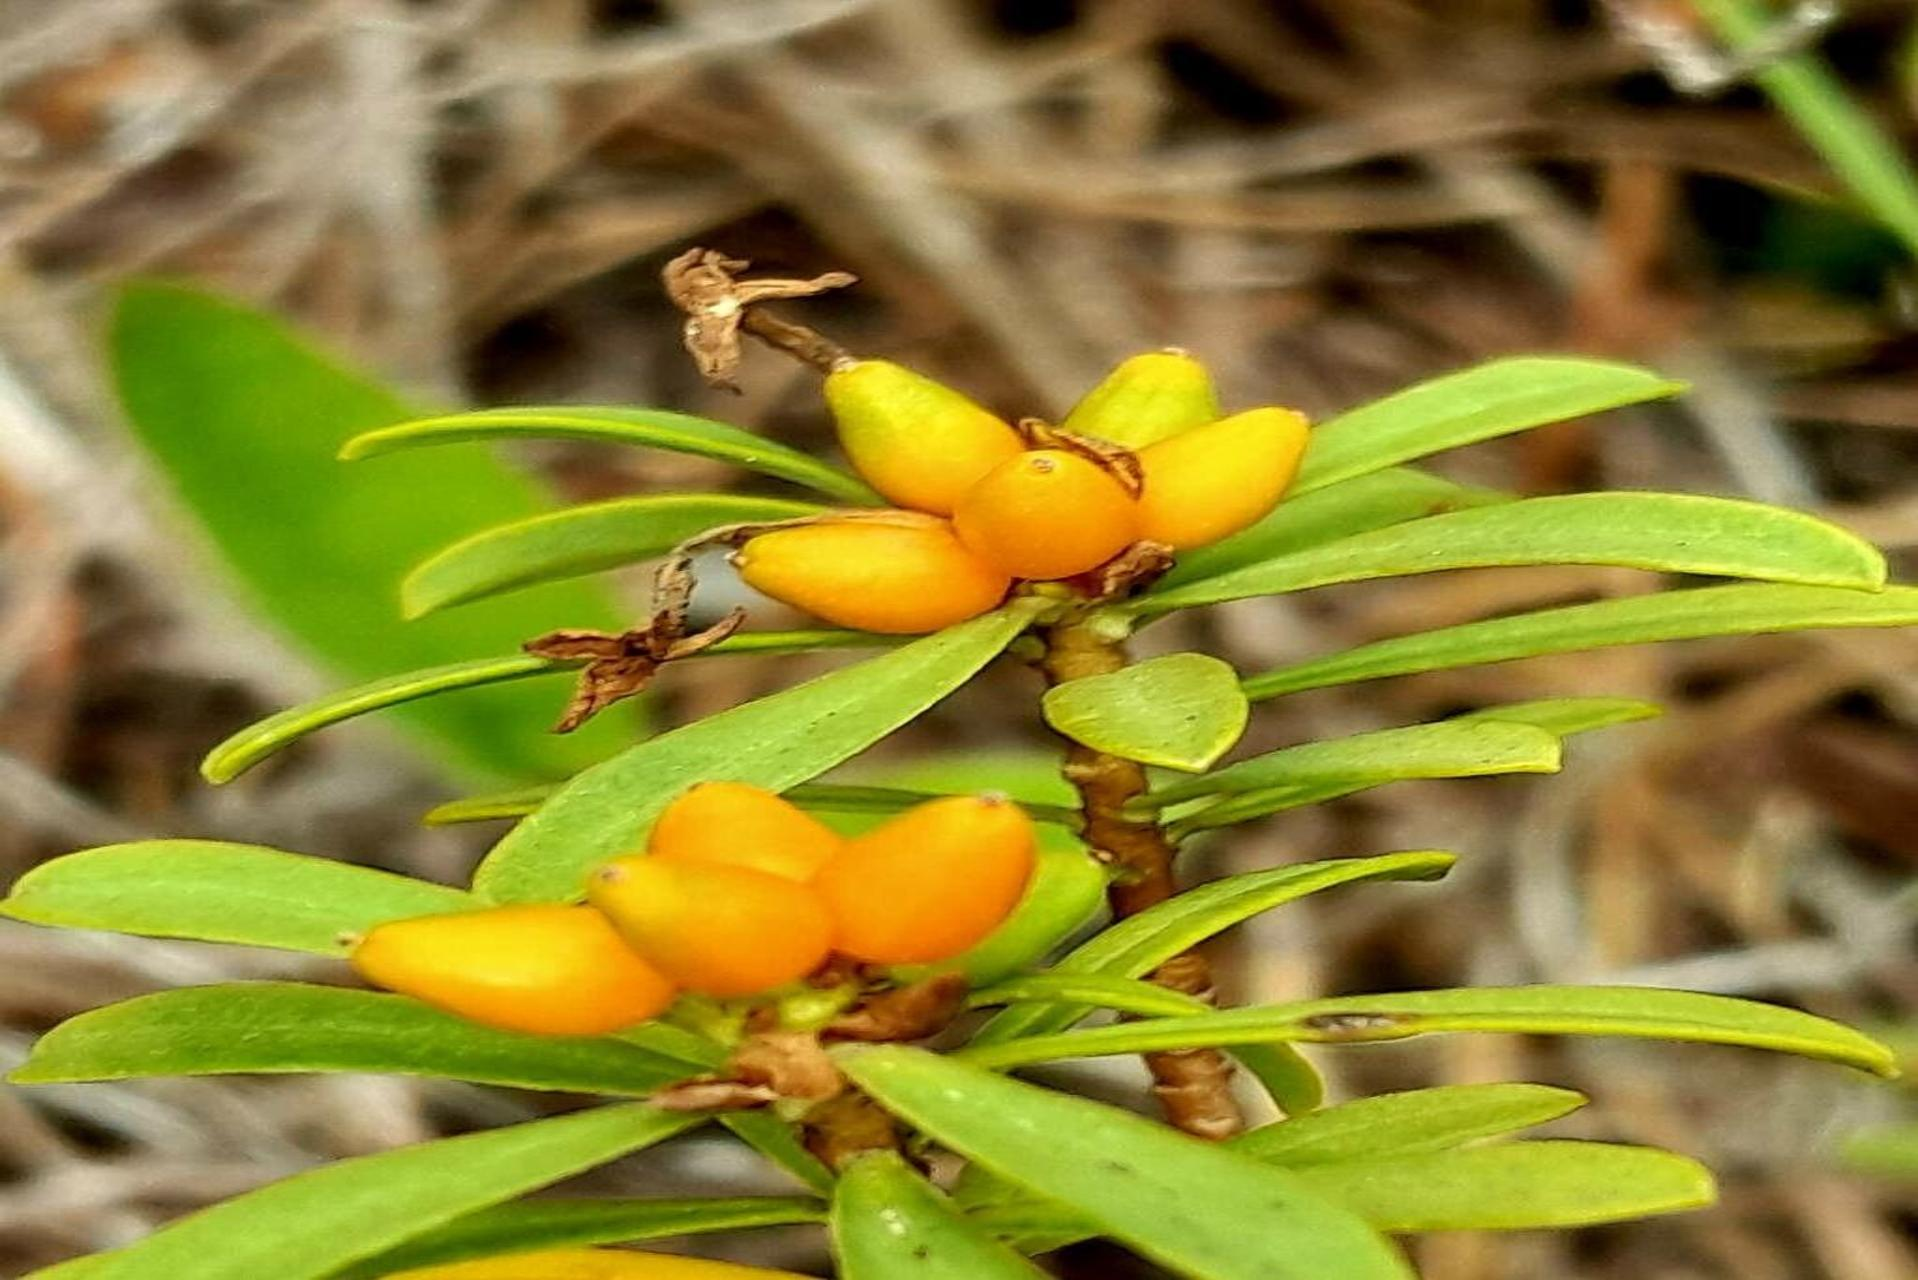
\includegraphics[width=0.9\linewidth]{images/daphne_striata.jpeg}
    \end{minipage}
    \caption{Malva sylvestris L. et Daphne striata Tratt.}
    \label{fig:malva}
\end{figure}

Ces observations préliminaires nous ont confirmé la nécessité d'une approche adaptative pour la présentation des résultats aux utilisateurs. En effet, un système qui proposerait un nombre fixe d'espèces candidates serait soit trop restrictif dans les cas difficiles (risquant d'oublier la bonne espèce), soit trop verbeux dans les cas simples (noyant l'utilisateur sous des propositions inutiles).

\vspace{0.2cm}
\vspace{0.2cm}

La prédiction conforme, que nous allons introduire dans la section suivante, offre plus précisément le cadre mathématique nécessaire pour adapter dynamiquement le nombre de suggestions en fonction de la difficulté de chaque cas d'identification.

%%%%%%%%%%%%%%%%%%%%%%%%%%%%%%%%%%%%%%%%%%%%%%%%%%%%%%%%%%%%%%%%%%%%%%%%%%%%%%%%

\subsection{Prédiction conforme}

La prédiction conforme est un cadre statistique qui permet de quantifier l'incertitude des prédictions faites par des algorithmes d'apprentissage automatique, y compris les réseaux de neurones utilisés dans Pl@ntNet. Contrairement aux autres approches comme le bootstrap qui reposent sur des hypothèses paramétriques, la prédiction conforme offre des garanties de couverture valables même pour des échantillons de taille finie, sans hypothèses fortes sur la distribution des données (\cite{ShaferVovk}).

\vspace{0.2cm}

\begin{figure}[H]
    \centering
    \begin{tabular}{@{}c@{\hspace{1mm}}c@{\hspace{1mm}}c@{}}
        % Première image et prédiction
        \begin{minipage}[t]{0.33\textwidth}
            \centering
            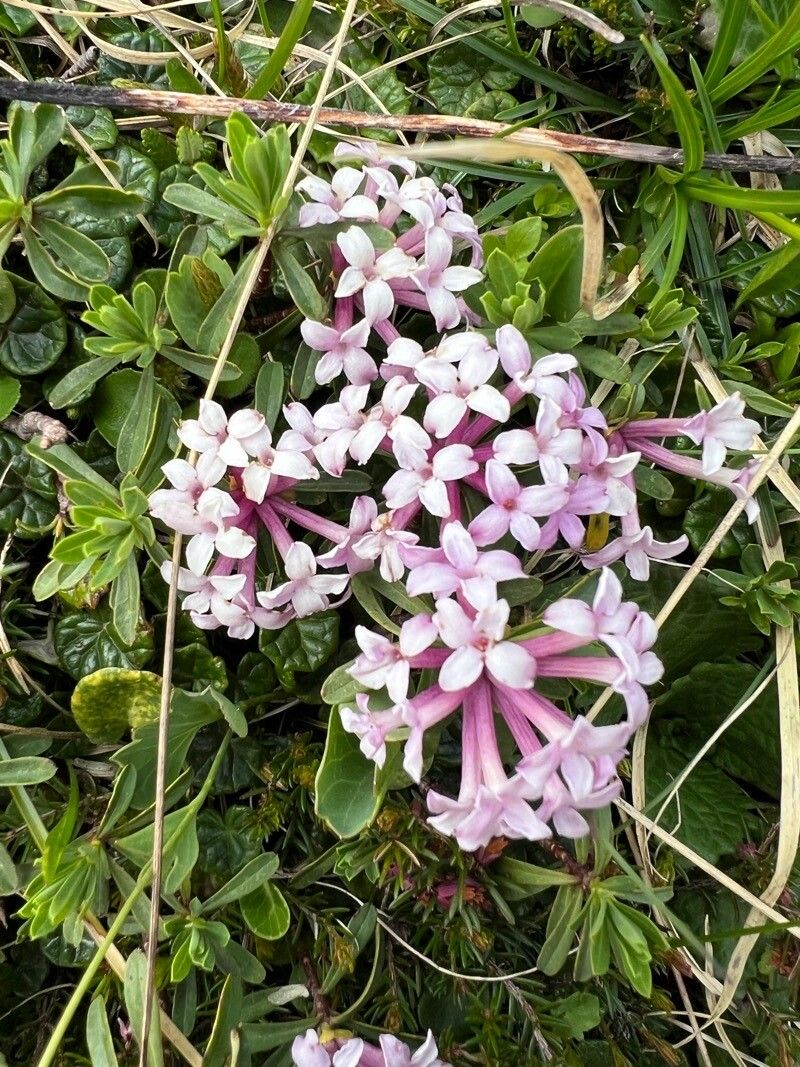
\includegraphics[width=\linewidth,height=4.5cm,keepaspectratio]{images/Daphne_1.jpeg}
            \[ \left\{ \begin{array}{@{}p{3.3cm}@{\hspace{2mm}}r@{}}
                \footnotesize\textcolor{magenta}{Daphne striata Tratt.} & \footnotesize 0,9556 \\
                \footnotesize Daphne cneorum L. & \footnotesize 0,0274 \\
                \footnotesize Daphne alpina L. & \footnotesize 0,0026
            \end{array} \right\} \]
        \end{minipage}
        & 
        % Deuxième image et prédiction
        \begin{minipage}[t]{0.33\textwidth}
            \centering
            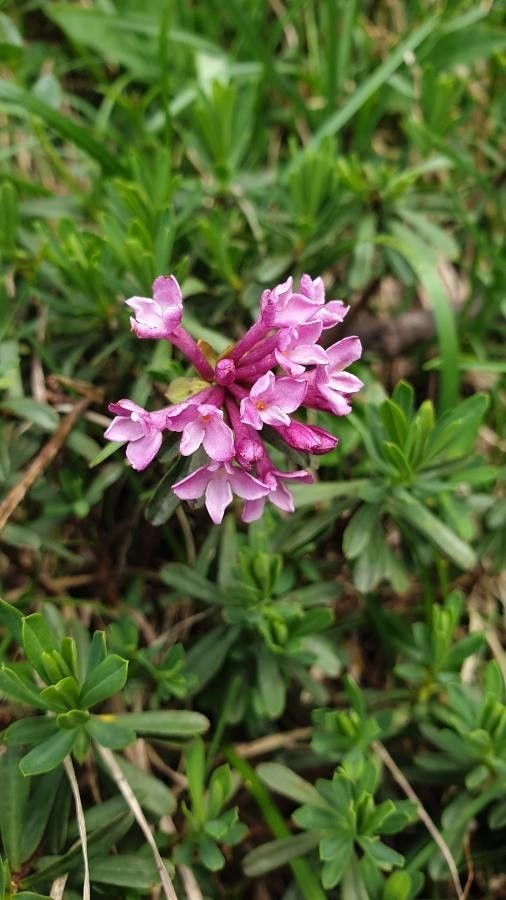
\includegraphics[width=\linewidth,height=4.5cm,keepaspectratio]{images/Daphne_2.jpeg}
            \[ \left\{ \begin{array}{@{}p{3.3cm}@{\hspace{2mm}}r@{}}
                \footnotesize\textcolor{magenta}{Daphne striata Tratt.} & \footnotesize 0,7547 \\
                \footnotesize Daphne cneorum L. & \footnotesize 0,2100 \\
                \footnotesize Daphne mezereum L. & \footnotesize 0,0045 \\
                \footnotesize Daphne alpina L. & \footnotesize 0,0020 \\
                \footnotesize Daphne sericea Vahl & \footnotesize 0,0014
            \end{array} \right\} \]
        \end{minipage}
        &
        % Troisième image et prédiction
        \begin{minipage}[t]{0.33\textwidth}
            \centering
            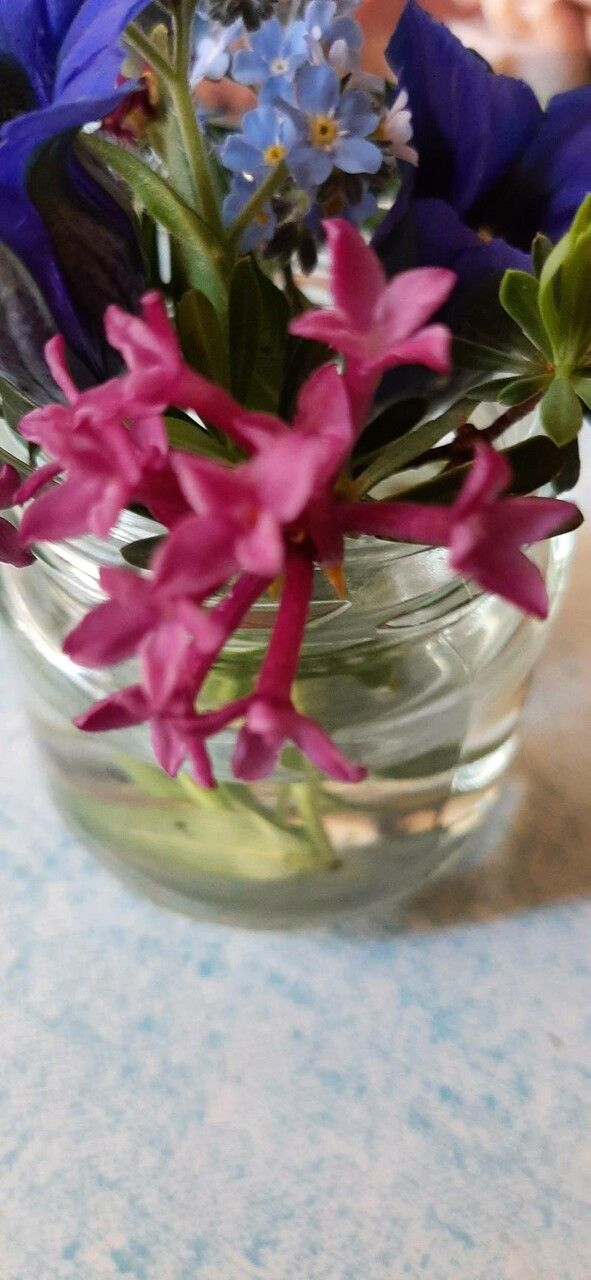
\includegraphics[width=\linewidth,height=4.5cm,keepaspectratio]{images/Daphne_3.jpeg}
            \[ \left\{ \begin{array}{@{}p{3.3cm}@{\hspace{2mm}}r@{}}
                \footnotesize Daphne cneorum L. & \footnotesize 0,6062 \\
                \footnotesize\textcolor{magenta}{Daphne striata Tratt.} & \footnotesize 0,3214 \\
                \footnotesize Daphne mezereum L. & \footnotesize 0,0040 \\
                \footnotesize Daphne alpina L. & \footnotesize 0,0033 \\
                \footnotesize Daphne laureola L. & \footnotesize 0,0012 \\
                \footnotesize Hyacinthus orientalis & \footnotesize 0,0011
            \end{array} \right\} \]
        \end{minipage}
    \end{tabular}
    \caption{Exemple d'ensembles de prédiction (c.-à-d., $C(X_{\text{test}})$) progressivement plus difficiles générés par prédiction conforme, sur des images de Pl@ntNet de la classe \textit{Daphne striata Tratt}.}
    \label{fig:prediction_sets}
\end{figure}

\subsubsection{Cadre mathématiques}

Nous considérons $(X_i, Y_i)$ des paires constituées de caractéristiques ($X_i$) et de réponses ($Y_i$) indépendantes et identiquement distribuées issues d'une distribution inconnue $P$, avec $i = 1, \dots, n$. Dans notre contexte, $X_i$ représente les caractéristiques extraites d'une image de plante, et $Y_i \in \{1, 2, \dots, K\}$ l'indice de la véritable espèce parmi les $K$ possibles. Notre espace des caractéristiques est $X = \mathbb R^d$ et notre espace des réponses est $Y = \mathbb R$.

\vspace{0.2cm}

L'objectif de la prédiction conforme est de construire, pour un nouvel échantillon $X_{n+1}$, un ensemble de prédiction $\hat{C}_n(X_{n+1}) \subseteq \{1, 2, \dots, K\}$ qui contienne la vraie classe $Y_{n+1}$ avec une probabilité d'au moins $1 - \alpha$, où $\alpha \in ]0,1[$ est un niveau d'erreur fixé à l'avance : 
$$ \mathbb P(Y_{n+1} \in \hat C_n (X_{n+1}) \geq 1 - \alpha) $$

\vspace{0.2cm}

Cette garantie de couverture est valable sous l'hypothèse que les paires $(X_i, Y_i)$ soient échangeables, une condition plus faible que l'indépendance et l'identité de distribution.

\vspace{0.2cm}

De plus, cela nécessite certaines conditions supplémentaires. La première va être de ne pas poser d'hypothèse sur $P$. Ensuite, nous ne devons pas non plus utiliser toutes les prédictions possibles, car nous voulons un nombre de prédictions fini, mais également raisonnable. Pour finir, nous voulons adapter notre stratégie à la dureté du problème, c'est-à-dire que plus il est facile de prédire $Y_{n+1}$ à partir de $X_{n+1}$ et plus notre ensemble $\hat C_n(X_{n+1})$ devra être petit, comme illustré en exemple dans la \hyperref[fig:prediction_sets]{\textcolor{purple}{figure 7}}.

\vspace{0.2cm}

Cela est tout à fait possible avec une distribution infinie dans des conditions standard (convergence du quantile de l'échantillon vers le quantile de la population). Mais, étant donné que nous sommes dans des conditions réelles, nous nous intéressons ici à des échantillons finis.

\subsubsection{Construction des ensembles de prédiction}

La construction des ensembles de prédiction conforme repose sur l'utilisation d'une fonction de score $s : \mathcal{X} \times \mathcal{Y} \rightarrow \mathbb{R}$ qui mesure la non-conformité (ou taux d'erreur) d'une paire (observation, classe). Plus cette valeur est élevée et moins l'observation et la classe sont conformes aux données d'entraînement.

\vspace{0.2cm}

La procédure de base comporte trois étapes : 
\begin{itemize}
    \item \textbf{Définition des vraies étiquettes :} pour les observations expertes, nous sommes partis du principe que, quand un expert avait donné une étiquette, elle était considérée comme correcte. Pour les observations non expertes, nous avons appliqué la méthode du vote majoritaire, que nous avons détaillé plus tôt, pour déterminer quel était le vrai label.
    \item \textbf{Calcul des scores de non-conformité :} pour chaque paire $(X_i, Y_i)$, on calcule un score $s(X_i, Y_i)$ qui indique à quel point cette paire est inhabituelle selon le modèle.
    \item \textbf{Construction de l'ensemble de prédiction :} pour un nouvel exemple $X_{n+1}$, on construit l'ensemble de prédiction en incluant toutes les classes $y$ pour lesquelles le score $s(X_{n+1}, y)$ est inférieur au quantile $(1- \alpha)$.
\end{itemize}

\vspace{0.2cm}

Cette procédure garantit que la probabilité que l'ensemble de prédiction contienne la vraie classe est d'au moins $1- \alpha$, c'est-à-dire $95\%$.

\subsubsection{Fonctions de scores}

Dans notre contexte de classification, plusieurs fonctions de score sont possibles. Nous avons donc choisi d'explorer deux principaux scores que sont la prédiction de la vraie classe et le score cumulatif.

\vspace{0.2cm}

Le score basé sur la probabilité de la vraie classe (\cite{Vovk}) se calcule comme suit : 
$$ s_1(X_i, Y_i) = 1 - p_{Y_i}(X_i) $$ où $p_{Y_i}(X_i)$ est la probabilité prédite par le modèle pour le vrai label. Plus cette probabilité est élevée et plus le score est faible, ce qui est souhaitable.

\vspace{0.2cm}

Le score cumulatif APS (Adaptive Prediction Sets) se calcule comme suit : 
$$ s_2(X_i, Y_i) = \sum_{j=1}^{r(X_i, Y_i)-1} p_{(j)}(X_i) $$ où $p_{(j)}(X_i)$ représente la $j$-ième plus grande probabilité prédite par le modèle pour l'observation $X_i$, et $r(X_i, Y_i)$ est le rang de la vraie classe $Y_i$ dans ce classement. Cette fonction de score, introduite par \cite{Romano}, permet de construire des ensembles de prédiction dont la taille s'adapte à la difficulté du problème.

\vspace{0.2cm}

Le score $s_2$ présente l'avantage de produire des ensembles de prédiction dont la taille varie en fonction de la confiance du modèle : pour les cas faciles où la vraie classe reçoit une probabilité dans celles les plus élevées (donc un rang faible), la somme sera petite et l'ensemble de prédiction contiendra peu de classes. Au contraire, pour les cas difficiles, l'ensemble sera plus grand pour maintenir la garantie de couverture.

%%%%%%%%%%%%%%%%%%%%%%%%%%%%%%%%%%%%%%%%%%%%%%%%%%%%%%%%%%%%%%%%%%%%%%%%%%%%%%%%

\subsection{Méthodologie d'évaluation et validation croisée}

Au-delà de la définition théorique des scores de non-conformité, nous avons dû concevoir une méthodologie pour évaluer l'efficacité de notre approche conforme. Pour garantir des résultats statistiquement valides, nous avons adopté une stratégie de division des données qui permet à la fois de calibrer nos modèles, mais également d'en tester les performances sur des échantillons indépendants pour pouvoir les comparer.

\subsubsection{Division des données}

Notre stratégie de division s'articule autour de deux critères principaux : l'expertise des utilisateurs et le type de score utilisé. Cette approche nous a conduit à créer quatre configurations distinctes : 
\begin{itemize}
    \item \textbf{Configuration $1$ :} score $s_1$ (probabilité de la vraie classe) avec calibration sur toutes les données non-expertes et test sur la moitié des données expertes.
    \item \textbf{Configuration $2$ :} score $s_1$ avec calibration sur la moitié des données expertes et test sur l'autre moitié des données expertes.
    \item \textbf{Configuration $3$ :} score $s_2$ (score cumulatif APS) avec calibration sur toutes les données non-expertes et test sur la moitié des données expertes.
    \item \textbf{Configuration $4$ :} score $s_2$ avec calibration sur la moitié des données expertes et test sur l'autre moitié des données expertes.
\end{itemize}

\vspace{0.2cm}

Nous avons représenté ces configurations comme suit : 
\begin{figure}[H]
    \centering
    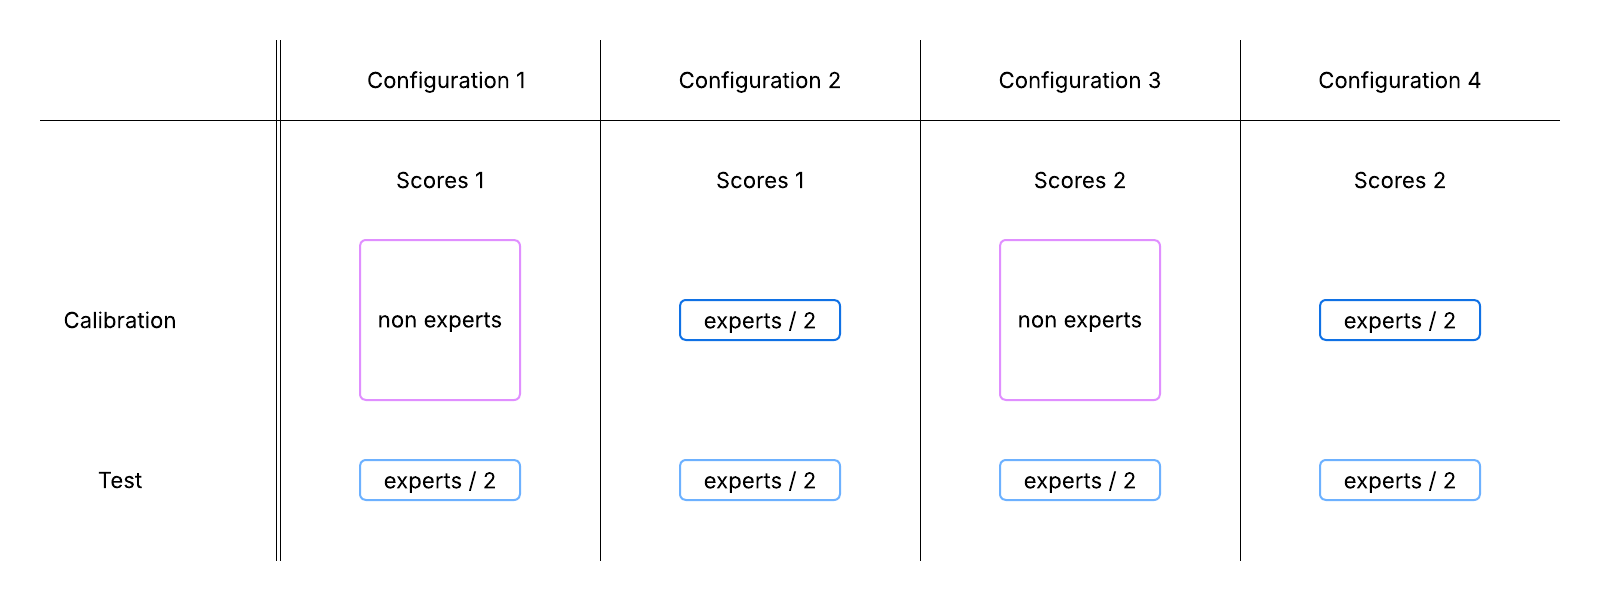
\includegraphics[scale=0.6]{images/Models.png}
    \caption{Représentation de nos quatre configurations}
    \label{models}
  \end{figure}

\vspace{0.2cm}

Cette structure nous permet d'évaluer non seulement l'impact du choix de la fonction de score ($s_1$ ou $s_2$), mais également l'influence de la qualité des données de calibration (expertes avec peu de données ou non expertes avec beaucoup de données) sur les performances finales.

\vspace{0.2cm}

Pour assurer la représentativité de nos échantillons, nous avons divisé les données expertes aléatoirement et avons vérifié que les deux groupes créés étaient bien similaires en termes de scores

\vspace{0.2cm}

Un léger problème s'est posé à nous après le calcul des scores. En effet, certaines observations présentaient des scores supérieurs à $1$, ce qui, s'agissant de valeurs dérivées de probabilités, n'est pas cohérent puisqu'ils devraient être compris entre $0$ et $1$. Après avoir examiné les quelques cas pour lesquels nous avons rencontré cette anomalie, nous avons constaté que ce phénomène n'apparaissait que pour les scores APS et uniquement pour des observations présentant des particularités au niveau de l'acquisition des données. Par exemple, nous avons identifié des cas où plusieurs plantes étaient présentes sur une même observation, ce qui engendrait une confusion pour l'algorithme qui ne pouvait déterminer avec précision quelle espèce identifier en priorité. Étant donné que ces cas problématiques étaient relativement rares ($149$ observations sur l'ensemble de notre échantillon de données), nous avons choisi de les exclure de notre analyse pour préserver l'intégrité de nos résultats.

\subsubsection{Calcul des quantiles}

Une fois les données divisées, l'étape suivante a consisté à calculer les quantiles des scores de non-conformité qui nous permettraient de construire nos ensembles de prédiction avec le niveau de garantie souhaitée de $95\%$.

\vspace{0.2cm}

Pour chaque configuration, nous avons commencé par récupérer les scores pour chaque observation du jeu de calibration que nous avons précédemment calculé. Puis, nous avons calculé le quantile à l'aide de la formule suivante : $$\frac{[(n+1)(1 - \alpha)]}{n}, \quad \text{avec } \alpha = 0,05$$ avec $\alpha$ qui représente notre niveau d'erreur souhaité et $n$ le nombre d'observations dans notre ensemble d'apprentissage. Enfin, nous avons implémenté une fonction qui, pour toute nouvelle observation, calcule les scores de non-conformité pour chaque classe possible et inclut dans l'ensemble de prédiction toutes les classes dont le score est inférieur au quantile calculé précédemment.

\vspace{0.2cm}

Pour le calcul concret du quantile, nous avons utilisé la fonction quantile de Python, adaptée pour notre large volume de données. Nous avons obtenu les résultats suivants : 

\begin{table}[H]
\centering
    \begin{tabular}{|l|c|}
        \hline
        \textbf{Configuration} & \textbf{Quantile calculé} \\
        \hline
        Score $s_1$ (soft max) + données non expertes & $0.9990$ \\
        Score $s_1$ + données expertes & $0.9649$ \\
        Score $s_2$ (APS) + données non expertes & $0.9990$ \\
        Score $s_2$ + données expertes & $0.7932$ \\
        \hline
        \end{tabular}
    \caption{Configuration des scores et des données avec les résultats de leurs quantiles}
    \label{tab: scores et quantiles}
\end{table}

\vspace{0.2cm}

Ces quantiles sont des seuils critiques, c'est-à-dire que pour le premier score (qui correspond au score soft max), nous incluons dans notre ensemble de prédiction toutes les classes dont le score est inférieur au quantile. Pour le deuxième scpre (qui correspond au score cumulatif APS), nous incluons les classes jusqu'à ce que leur somme cumulée dépasse le quantile.

\begin{figure}[H]
    \centering
        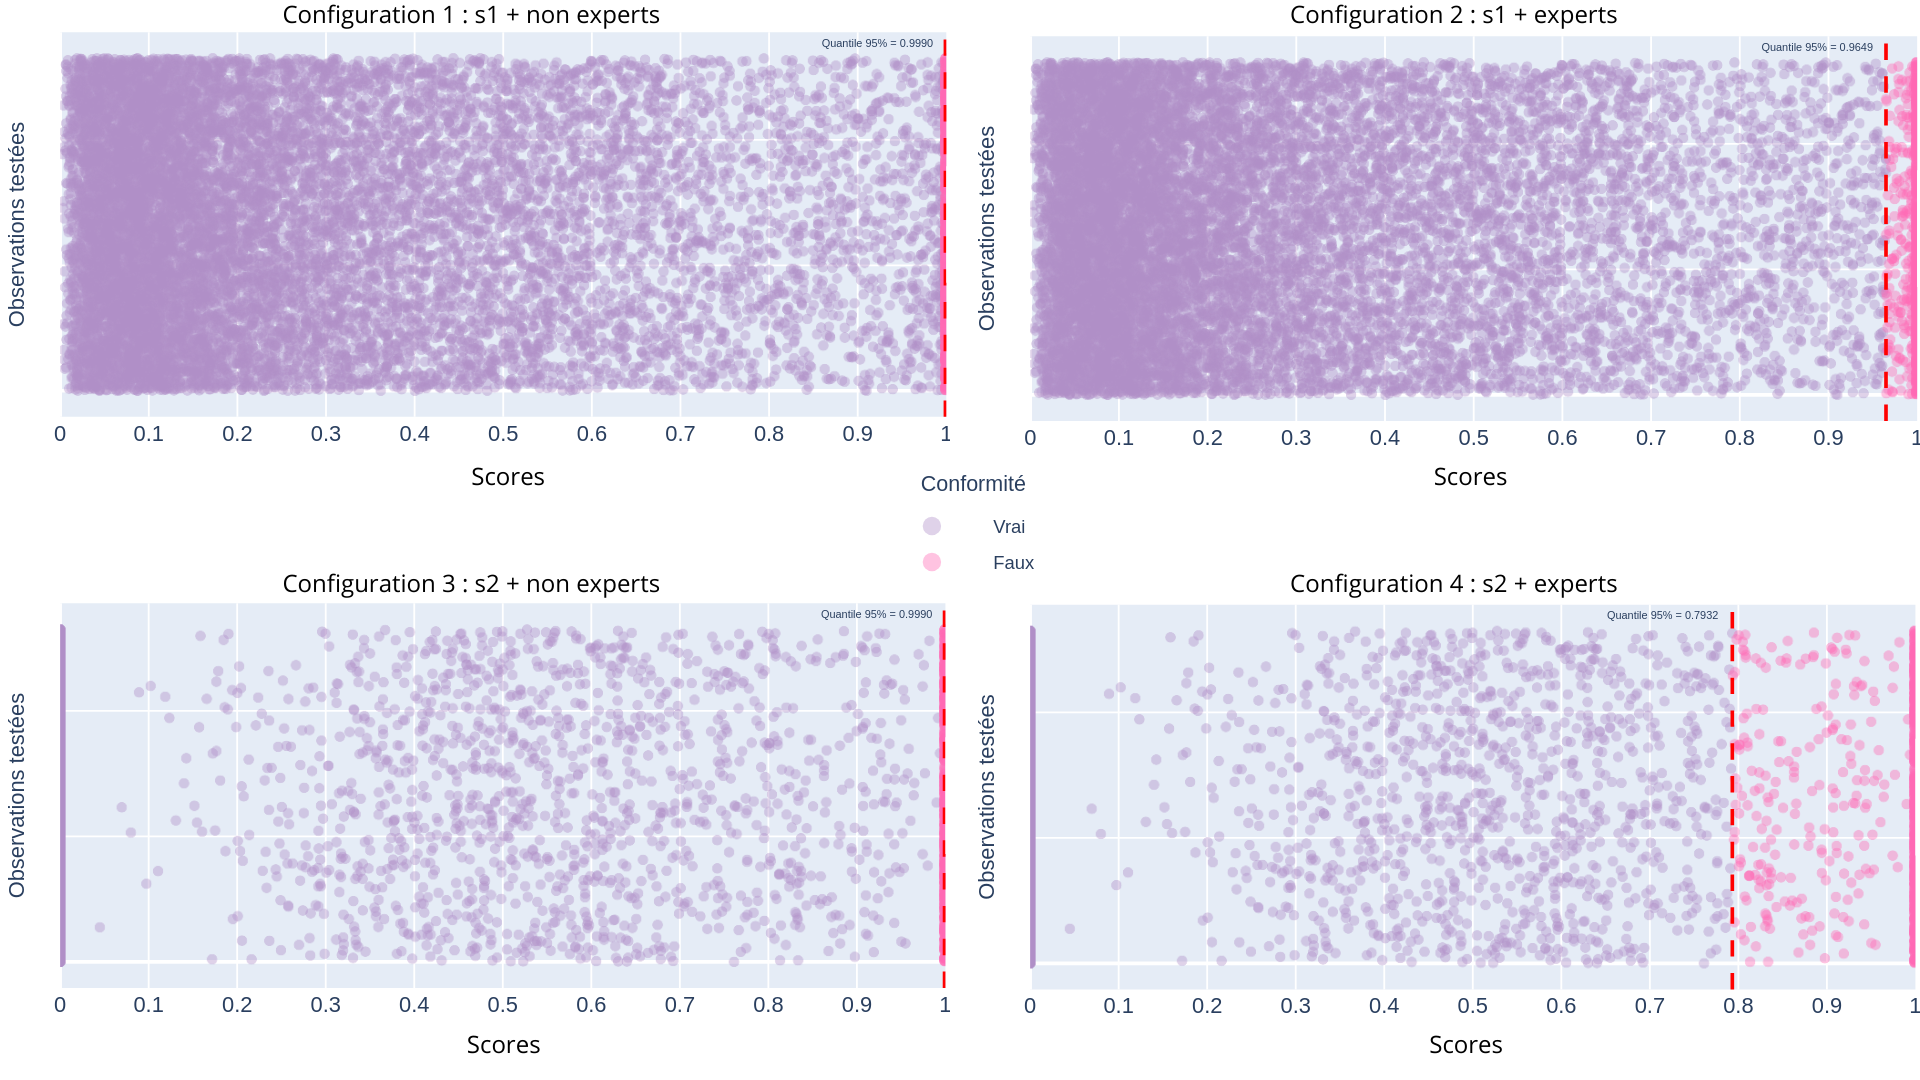
\includegraphics[width=1\linewidth]{images/quantiles.png}
    \caption{Conservation des observations en fonction des quantiles des configurations}
    \label{fig:quantiles}
\end{figure}

Analysons le \hyperref[tab: scores et quantiles]{\textcolor{purple}{tableau 2}} ainsi que la \hyperref[fig:quantiles]{\textcolor{purple}{figure 9}} associée.
Ce tableau présente les quantiles calculés pour chaque configuration de score ($s_1$ ou $s_2$) et de type de données (expertes ou non expertes).

\vspace{0.2cm}

Il est important de noter que les quantiles obtenus pour $s_1$ et $s_2$ ne sont pas directement comparables, car ces scores se calculent de manière différentes et sont définis sur des échelles distinctes. Mais il vont nous servir par la suite à définir nos ensembles de prédiction et pouvoir comparer nos configurations.

\vspace{0.2cm}

Autrement dit, un quantile plus bas pour $s_2$ ne signifie pas nécessairement une méthode plus stricte que $s_1$, mais reflète plutôt la nature différente du score. C’est pourquoi l’interprétation doit se faire au sein d’un même score, en comparant les données expertes vs non expertes.

\vspace{0.2cm}

Ces résultats soulignent le rôle des quantiles comme seuil critique dans la prise de décision. Un quantile élevé reflète une tolérance accrue aux écarts (donc une confiance moindre dans la sélection), tandis qu’un quantile plus bas indique une sélection plus exigeante. Chaque score ajuste ainsi la sensibilité du modèle selon le type de données utilisées.

\vspace{0.2cm}

La \hyperref[fig:quantiles]{\textcolor{purple}{figure 9}} illustre la répartition des observations testées selon les scores $s_1$ et $s_2$, en distinguant les données expertes et non expertes. L’axe des abscisses représente les types de score, tandis que l’axe des ordonnées indique les scores de non-conformité calculés pour chaque observation testée. Chaque point correspond à une observation : la valeur affichée représente le score de non-conformité associé à la vraie espèce (le bon label) pour cette observation. La ligne rouge en pointillé marque le seuil du quantile utilisé pour la prédiction conforme. Les couleurs différenciées permettent de visualiser la conformité des observations : en violet les observations conformes (c’est-à-dire dont la vraie espèce est incluse dans l’ensemble de prédiction), en rose celles jugées non conformes.

\vspace{0.2cm}

Donc, nous pouvons voir que le score $s_2$ tend à réduire la proportion d’observations acceptées, en particulier lorsqu’il est appliqué aux données expertes.

\vspace{0.2cm}

En conclusion, ces résultats démontrent que le choix du score ainsi que la nature des données influencent de manière significative le processus de sélection des observations.

\vspace{0.2cm}

Une fois ces quantiles obtenus, nous avons pu les utiliser afin de tester la validité de notre modèle.

\subsubsection{Test sur nos données expertes}

Pour évaluer l'efficacité de notre approche de prédiction conforme, nous avons mesuré deux métriques principales que sont le taux de couverture et leurs tailles (moyenne et médiane) que nous avons calculé sur nos ensembles de prédiction construit à partie de nos données de test. 

\vspace{0.2cm}

Le taux de couverture représente la proportion des observations pour lesquelles la vraie classe est incluse dans l'ensemble de prédiction. Idéalement, ce taux devrait être aux alentours de $1- \alpha$, c'est-à-dire à $95\%$.

\vspace{0.2cm}

De plus, nous avons calculé la taille moyenne des ensembles de prédiction, qui correspond au nombre moyen de classes proposées pour chaque observation. Pour une meilleure expérience utilisateur, cette taille doit être la plus petite possible parmi les ensembles non vides, pour garantir une réponse concise et pertinente à l'utilisateur, tout en maintenant une couverture adéquate.

\vspace{0.2cm}

Les résultats que nous avons obtenus seront détaillés dans la partie suivante, afin de pouvoir comparer nos modèles en même temps.

%%%%%%%%%%%%%%%%%%%%%%%%%%%%%%%%%%%%%%%%%%%%%%%%%%%%%%%%%%%%%%%%%%%%%%%%%%%%%%%%
%%%%%%%%%%%%%%%%%%%%%%%%%%%%%%%%%%%%%%%%%%%%%%%%%%%%%%%%%%%%%%%%%%%%%%%%%%%%%%%%

\section{Résultats et discussion}

Après avoir défini notre méthodologie et implémenté les algorithmes correspondants, nous avons procédé à l'évaluation systématique des quatre configurations décrites précédemment à l'aide des variables calculées. Cette section présente les résultats obtenus, analyse leurs implications en pratique et discute de la généralisation de notre approche à l'ensemble des données Pl@ntNet.

%%%%%%%%%%%%%%%%%%%%%%%%%%%%%%%%%%%%%%%%%%%%%%%%%%%%%%%%%%%%%%%%%%%%%%%%%%%%%%%%

\subsection{Analyse comparative}

À la suite de nos calculs pour mesurer l'efficacité de nos modèles, les résultats obtenus pour nos quatre configurations sont résumés dans le tableau suivant :

\begin{table}[H]
\centering
\begin{tabular}{|l|c|c|c|}
    \hline
    \textbf{Configuration} & \textbf{Taux de couverture} & \textbf{Taille moyenne} & \textbf{Taille médiane} \\
    \hline
    $s_1$ (Softmax) + non expert & $96.45\%$ & $15.47$ & $10.00$ \\
    $s_1$ + expert & $94.82\%$ & $2.13$ & $2.00$ \\
    $s_2$ (APS) + non expert & $96.45\%$ & $11.21$ & $7.00$ \\
    $s_2$ + expert & $94.76\%$ & $4.51$ & $2.00$ \\
    \hline
    \end{tabular}
\caption{Configuration et caractéristiques obtenues (couverture, tailles moyenne et médiane)}
\label{tab3}
\end{table}
    
Ces résultats révèlent plusieurs tendances importantes concernant l'effet du score choisi ($s_1$ vs $s_2$) et de la nature des données de calibration (expertes vs non-expertes) sur les performances finales du modèle.

\vspace{0.2cm}

Les configurations basées sur les données non-expertes ont tendance à produire des ensembles de prédiction couvrant plus de bon labels que ce que nous avions défini, ce qui pourrait indiquer que les scores de test (experts) ne se comportent pas de la même manière que ceux de la calibration (non experts). Les calibrations avec données expertes respectent le taux de couverture que nous nous étions fixé (de $95\%$), reflétant une meilleure qualité de calibration malgré la taille d’échantillon plus réduite. Nous vérifierons si le taux de couverture est significativement différent du taux attendu de $95\%$, à l’aide d’un test du Chi-deux, plus tard dans notre rapport.

\vspace{0.2cm}

Si nous cherchons à comparer nos deux scores, nous pouvons voir qu'il y a une différence au niveau de la taille moyenne et médiane des ensembles de prédiction. En effet, nous pouvons voir que, lorsque nous utilisons les données non expertes en tant que données de calibration, nous obtenons des tailles d'ensemble bien plus importante que lorsque nous utilisons les données expertes, pouvant ainsi expliquer en partie pourquoi nous obtenons des taux de couvertures plus importants dans ces cas-là. De plus, nous voyons que les tailles médianes sont similaires pour les configurations $2$ et $4$. Le fait que le nombre de label par observations soit de $2$ pour la médiane nous indique que les tailles semblent raisonnable et qu'il n'y a pas besoin d'un nombre de label très important pour respecter le taux de couverture attendu, ce qui est une bonne chose.

\vspace{0.2cm}

Pour essayer de comparer l'utilisation de l'un ou l'autre des scores, nous pouvons dire que les tailles moyennes sont différentes, avec celle de la configuration $4$ près de deux fois supérieure à celle de la deuxième. Cela pourrait s'expliquer par le fait qu'il y a sûrement des valeurs extrêmes avec un nombre de label très important pour certaines observations, ce qui fait monter la moyenne mais en laissant la médiane similaire.

\vspace{0.2cm}

Si nous devions conclure sur une configuration optimale, nous prendrons les groupes de calibration et les groupes de test pour les données expertes. En ce qui concerne le score, les deux semblent donner des ensembles cohérents mais nous privilégierons le premier score (soft max) pour sa taille moyenne inférieure à celle du score APS.

%%%%%%%%%%%%%%%%%%%%%%%%%%%%%%%%%%%%%%%%%%%%%%%%%%%%%%%%%%%%%%%%%%%%%%%%%%%%%%%%

\subsection{Analyse de la robustesse au tirage aléatoire}

Pour vérifier si la division aléatoire des données a influencé les performances, nous avons répété notre expérience avec plusieurs autres graines ($123$ et $545$). Les résultats présentés dans le \hyperref[tab3]{\textcolor{purple}{tableau 3}} ci-dessus proviennent de la graine $42$. Les performances obtenues pour les méthodes calibrées sont présentées ci-dessous :

\begin{table}[h]
    \centering
    \begin{tabular}{|l|c|c|c|c|}
        \hline
        \textbf{Configuration} & \textbf{Graine $42$} & \textbf{Graine $123$} & \textbf{Graine $545$} & \textbf{Ecart-max} \\
        \hline
        $s_1$ + non expert & $96.45\%$ & $96.52\%$ & $96.66\%$ & $0.21\%$ \\
        $s_1$ + expert & $94.82\%$ & $94.95\%$ & $95.15\%$ & $0.33\%$ \\
        $s_2$ + non expert & $96.45\%$ & $96.52\%$ & $96.66\%$ & $0.21\%$ \\
        $s_2$ + expert & $94.76\%$ & $95.01\%$ & $95.24\%$ & $0.48\%$ \\
        \hline
    \end{tabular}
    \caption{Résumé des couvertures avec les différentes graines}
    \label{tab:couvertures_graines}
\end{table}

Les taux de couverture obtenus varient très peu selon le choix de la graine utilisée pour couper les données expertes. En effet, nous observons un écart maximal observé de $0,48\%$. De plus, les méthodes calibrées sur les non-experts restent systématiquement au-dessus de $95\%$ et les méthodes calibrées sur les experts restent très proches de $95\%$, sans variation notable.

\vspace{0.2cm}

Donc nous pouvons remarquer que les résultats sont robustes au split aléatoire des données expertes. Ainsi, le choix de la graine n’affecte pas significativement les taux de couverture, ce qui confirme que la calibration sur une moitié raisonnablement tirée des experts donne des résultats stables.

\subsection{Validation statistique des taux de couverture (test du $\chi^2$)}

Afin de confirmer si les taux de couverture observés respectaient réellement la garantie théorique de $95\%$, nous avons appliqué un test statistique du Chi-deux ($\chi^2$) d’adéquation pour chaque méthode. L’hypothèse nulle $(H_0)$ stipule que le taux de couverture est égal à $95\%$ contre l'hypothèse $(H_1)$ qui stipule que le taux de couverture est différent de $95\%$. Le seuil que nous appliquons ici pour déterminer si nous conservons ou rejetons $(H_0)$ est de $3,8415$. Voici un résumé des résultats obtenus pour chaque configuration :

\begin{table}[H]
    \centering
    \begin{tabular}{|l|c|c|c|c|}
        \hline
        \textbf{Configuration} & \textbf{Statistique $\chi^2$} & \textbf{Test} & \textbf{Conclusion} \\
        \hline
        $s_1$ + non expert & $58.90$ & $> 3.8415$ & Rejet de $H_0$ (supérieure au seuil) \\
        $s_1$ + expert & $0.87$ & $< 3.8415$  & Conservation de $H_0$ \\
        $s_2$ + non expert & $58.90$ & $> 3.8415$ & Rejet de $H_0$ (supérieure au seuil) \\
        $s_2$ + expert & $1.57$ & $< 3.8415$ & Conservation de $H_0$ \\
        \hline
    \end{tabular}
    \caption{Résumé des tests de $\chi^2$}
    \label{tab:Tests du Chi-2}
\end{table}

Ces résultats montrent que, lorsque la calibration est effectuée sur des données non expertes, la couverture obtenue est significativement trop élevée, trahissant une surestimation du quantile. À l’inverse, les calibrations effectuées sur des données expertes respectent bien la garantie de $95\%$ et passent le test sans rejeter $H_0$, validant ainsi la bonne calibration.

\subsection{Perspectives d'intégration dans l'application}

\subsubsection{Implémentation dans l'application}

L'objectif de ce travail est de rendre l'utilisation de l'application bien plus pratique pour les utilisateurs. Cela peut se faire grâce à plusieurs ajustements.

\vspace{0.2cm}

Dans un premier temps, nous pourrions nous baser sur les quantiles que nous avons calculé (avec le deuxième score et les données expertes) afin de ne conserver que les prédictions d'espèces dont la probabilité dépasse le $1 -$ quantile. Ainsi, l'utilisateur aurait un nombre d'espèces proposées bien moins important et il lui serait plus facile et plus rapide de vérifier quelle proposition lui semble adéquat avec la plante qui se trouve devant lui.

\vspace{0.2cm}

Si nous reprenons l'exemple de la \hyperref[fig:prediction_sets]{\textcolor{purple}{figure 7}}, alors nous obtiendrons une taille de une seule espèce prédite pour chacune des observations. Cela s'explique par le fait qu'il n'y a que la première prédiction dont la probabilité était supérieure à $1 - 0,5614$. Cependant, pour la dernière plante, étant donné que la photographie est de mauvaise qualité, ce n'est pas la bonne espèce qui est prédite (elle fait partie de $5\%$ d'erreur).

\vspace{0.2cm}

Dans un second temps, il serait intéressant que l'utilisateur puisse choisir le taux de couverture qu'il souhaite en fonction de la situation dans laquelle il se trouve, et donc, en fonction de ce qu'il choisit, que le nombre d'espèces proposées s'adapte. 

\vspace{0.2cm}

Par exemple, un utilisateur pressé pourrait vouloir un taux de couverture de $90\%$ (donc un quantile relativement faible), c'est-à-dire ne pas être certain d'avoir la bonne espèce mais avoir un nombre de proposition limité (seulement celles avec une probabilité $> 1 -$ quantile). D'un autre côté, un utilisateur qui veut absolument savoir précisément quelle plante il a devant lui pourrait sélectionner un taux de couverture de $99\%$ (donc un quantile très élevé), c'est-à-dire qu'il aura un nombre d'espèce élevé (même celles avec des faibles probabilités), ainsi il pourra vérifier à la main quelle plante il pense avoir devant lui et toutes celles probables lui seront proposées.

\vspace{0.2cm}

Si le temps l'avait permis, nous aurions souhaité développer un exemple d'interface utilisateur intégrant notre système de prédiction conforme, afin de démontrer concrètement l'amélioration potentielle de l'expérience utilisateur.

\subsubsection{Ouverture}

Si nous devions donner des perspectives d'amélioration à notre travail, il aurait été intéressant de calculer un quantile pour chaque espèce ou, au moins, pour chaque famille de plante. En effet, le taux de couverture de $95\%$ est une moyenne globale mais, étant donné que nous avons énormément de plantes, il se pourrait que certaines espèces soient bien plus faciles à reconnaître et donc que leur quantile soit bien plus élevé que certaines plantes peu observées ou difficiles à reconnaître. Ainsi, cela permettrait de pouvoir encore plus adapter le nombre de prédictions en fonction de l'observation.

\vspace{0.2cm}

De plus, nos calculs pourraient être effectués pour les données provenant d'autres régions du monde et plus uniquement sur les données d'Europe du Sud-Ouest que nous avons traitées.

%%%%%%%%%%%%%%%%%%%%%%%%%%%%%%%%%%%%%%%%%%%%%%%%%%%%%%%%%%%%%%%%%%%%%%%%%%%%%%%%
%%%%%%%%%%%%%%%%%%%%%%%%%%%%%%%%%%%%%%%%%%%%%%%%%%%%%%%%%%%%%%%%%%%%%%%%%%%%%%%%

\section{Conclusion}

Dans ce projet, nous avons abordé la problématique de l'incertitude dans l'identification automatique des plantes, un défi majeur pour l'application Pl@ntNet qui repose sur des données collectées par une vaste communauté d'utilisateurs aux expertises avérées. Notre approche s'est articulée autour de la prédiction conforme, un cadre statistique qui permet de transformer des sorties probabilistes d'un modèle de classification en ensembles de prédiction dotés de garanties de couverture.

\vspace{0.2cm}

À partir d'un jeu de données de plus de $6$ millions d'observations d'espèces végétales en Europe du Sud-Ouest, nous avons développé une méthodologie permettant d'adapter dynamiquement le nombre de suggestions d'espèces en fonction de la difficulté d'identification de chaque image. 

\vspace{0.2cm}

Cette approche présente plusieurs avantages par rapport au système actuel de Pl@ntNet, notamment parce qu'elle fournit une garantie statistique que la vraie espèce est incluse dans l'ensemble des suggestions avec une probabilité d'au moin $95\%$. De plus, elle réduit le nombre de suggestions dans les cas faciles, tout en élargissant les propositions dans les cas ambigus pour maintenir la garantie de couverture.

\vspace{0.2cm}

Nos expériences ont démontré l'importance de la qualité des données de calibration. La configuration combinant le score de la vraie classe avec une calibration sur données expertes a produit les résultats les plus convaincants, avec une taille médiane d'ensemble de prédiction de $2$, tout en maintenant le taux de couverture proche de $95\%$.

\vspace{0.2cm}

De plus, les tests statistiques ont confirmé que les calibrations basées sur les experts respectaient bien la garantie théorique de couverture de $95\%$, contrairement à celles basées sur les données non expertes, qui ont montré une surcouverture systématique. L’analyse sur différentes graines de division a également démontré la stabilité et la robustesse de nos résultats vis-à-vis de la composition du jeu de calibration.

\vspace{0.2cm}

Ce projet ouvre plusieurs perspectives intéressantes pour des travaux futurs, notamment l'élargissement de nos travaux aux données d'autres secteurs géographiques, l'intégration de notre travail pour améliorer l'interface utilisateur dans l'application ainsi que l'adaptation des quantiles à des espèces ou des familles d'espèces.

\vspace{0.2cm}

En conclusion, notre étude démontre le potentiel de la prédiction conforme pour améliorer la fiabilité et l'expérience utilisateur des systèmes d'identification automatique des plantes, et plus généralement, de tout système de classification automatique confronté à des données de qualité variable et à des situations d'ambiguïté naturelle.

\printbibliography

\end{document}

